% =====================================================================
% Paper JSAC v3
% Body digital twin for exposure-constrained mmWave downlink under
% European reference-level regulation. Multi-body MMSE-with-exposure
% precoder with primal projection, scene path dictionary, virtual-IMU
% pose telemetry, binding-regime plaza-scale evaluation.
%
% Author: Robin Wydaeghe
% Target: IEEE JSAC SI on Digital Twins for Wireless Networks (Q4 2026)
% =====================================================================

\documentclass[journal,twocolumn,10pt]{IEEEtran}

\usepackage[utf8]{inputenc}
\usepackage[T1]{fontenc}
\usepackage{lmodern}
\usepackage{microtype}

\usepackage{amsmath,amssymb,amsthm,mathtools}
\usepackage{bm}

\usepackage{graphicx}
\graphicspath{{../../papers/drafts/figures/}{../../theory/figures/}{../../validation/}{../../JSAC/code/experiments/rank_check/}{../../JSAC/code/experiments/cauchy_tightness/}{../../JSAC/code/experiments/csi_calibration/}{../../JSAC/code/experiments/tier_c_decision/}{../../JSAC/code/experiments/plaza_run/figures/}}
\usepackage{booktabs}
\usepackage{array}
\usepackage{multirow}
\usepackage{caption}
\usepackage{subcaption}

\usepackage{cite}
\usepackage{xcolor}
\usepackage[colorlinks=true,linkcolor=blue,citecolor=blue,urlcolor=blue]{hyperref}
\usepackage[capitalize,nameinlink]{cleveref}

\theoremstyle{plain}
\newtheorem{theorem}{Theorem}
\newtheorem{proposition}[theorem]{Proposition}
\newtheorem{corollary}[theorem]{Corollary}
\theoremstyle{remark}
\newtheorem{remark}[theorem]{Remark}

\crefname{proposition}{Proposition}{Propositions}
\Crefname{proposition}{Proposition}{Propositions}
\crefname{corollary}{Corollary}{Corollaries}
\Crefname{corollary}{Corollary}{Corollaries}
\crefname{remark}{Remark}{Remarks}
\Crefname{remark}{Remark}{Remarks}
\crefname{theorem}{Theorem}{Theorems}
\Crefname{theorem}{Theorem}{Theorems}

\newcommand{\khat}{\hat{\bm{k}}}
\newcommand{\nhat}{\hat{\bm{n}}}
\newcommand{\rr}{\mathbf{r}}
\newcommand{\xx}{\mathbf{x}}
\newcommand{\hh}{\mathbf{h}}
\newcommand{\ww}{\mathbf{w}}
\newcommand{\gvec}{\mathbf{g}}
\newcommand{\bvec}{\mathbf{b}}
\newcommand{\Sinc}{S_{\mathrm{inc}}}
\newcommand{\Sab}{S_{\mathrm{ab}}}
\newcommand{\Pabs}{P_{\mathrm{abs}}}
\newcommand{\Aab}{A_{\mathrm{ab}}}
\newcommand{\GG}{\mathbf{G}}
\newcommand{\Gtil}{\tilde{\mathbf{G}}}
\newcommand{\Qmat}{\mathbf{Q}}
\newcommand{\Mmat}{\mathbf{M}}
\newcommand{\Hintf}{\mathbf{H}_{\mathrm{intf}}}
\newcommand{\Jmat}{\mathbf{J}}
\newcommand{\HH}{\mathbf{H}}
\newcommand{\WW}{\mathbf{W}}
\newcommand{\II}{\mathbf{I}}
\newcommand{\PabsZF}{P_{\mathrm{abs},\mathrm{ZF}}}
\newcommand{\Phimat}{\mathbf{\Phi}}
\newcommand{\Psimat}{\bm{\Psi}}
\newcommand{\Psitil}{\tilde{\bm{\Psi}}}
\newcommand{\Fn}{\mathbf{F}_n}
\newcommand{\psin}{\bm{\psi}_n}
\newcommand{\diff}{\mathrm{d}}
\newcommand{\Complex}{\mathbb{C}}
\newcommand{\ntilde}{\tilde{n}}
\newcommand{\AllBodies}{\mathcal{P}}
\newcommand{\Served}{\mathcal{U}}
\newcommand{\Bystanders}{\mathcal{B}}
\newcommand{\Dict}{\mathcal{D}}
\DeclareMathOperator{\ReLU}{ReLU}
\DeclareMathOperator{\RE}{Re}
\DeclareMathOperator{\IM}{Im}
\DeclareMathOperator{\tr}{tr}

\title{Body Digital Twins for Exposure-Constrained mmWave Downlink:
A Multi-Body QCQP under European Reference Levels}

\author{Robin~Wydaeghe%
  \thanks{R. Wydaeghe is with Ghent University and imec, Ghent, Belgium
  (e-mail: robin.wydaeghe@ugent.be).}}

\markboth{IEEE Journal on Selected Areas in Communications,
  Vol.~XX, No.~X, Month~2026}%
{Wydaeghe: Body digital twins for exposure-constrained mmWave downlink}

\begin{document}

\maketitle

\begin{abstract}
European reference-level caps on the electromagnetic field, including
the post-2014 Brussels arrêté at $14.57\,$V/m and the Italian
attention values at $3$-$6\,$V/m under the 2024 decree, can bind
millimetre-wave downlink at high transmit power before propagation
does. We bring per-body absorbed power into the precoder loop by
maintaining a digital twin per body that returns whole-body absorbed
power as a Hermitian quadratic form $\Pabs^{(u)} = \xx^H \Qmat^{(u)}
\xx$, factoring $\Qmat^{(u)} = \Jmat^T \Mmat^{(u)} \Jmat$ so the
array-hardware combinatorics separate from a body-and-scene Gram, and
building the scene-side path set once on a static dictionary
refreshed under body translation by a diagonal phasor. Tiered
telemetry covers served users, cooperating non-users, ISAC-sensed
bystanders, and undetected occupancy; IMU-bearing tiers carry a
virtual inertial-mocap pose at $4^\circ$ per-joint RMS attitude
error. We then show that under the 3GPP NR FR2 MCS28 spectral-efficiency
cap of $7.4\,$bps/Hz (which a regularised zero-forcing precoder on
a tens-of-element panel saturates with substantial SINR margin), the
multi-body sum-rate-maximisation QCQP under per-body caps admits a
one-line per-slot closed-form optimum: the primal projection of
regularised ZF, $\ww_k \leftarrow \alpha\,\ww_k$ with $\alpha =
\min(1, \sqrt{\eta_S \min_u L^{(u)}/\Pabs^{(u)}})$, saturates the
$K + B$ per-body caps and the per-stream MCS cap simultaneously,
without any inner optimiser. The projection is feasible by
construction at $\eta_S \in (0, 1]$ and costs $O(B M r)$ per slot at
low rank $r$ of the body-coupling Gram. We instantiate the loop on
a Brussels Grand Place geometry with 50 SMPL-X bodies, an $8 \times
8$ panel at $26\,$GHz, 25 served users, $43\,$dBm conducted, and
$E_{\mathrm{RL}} = 3\,$V/m. Regularised ZF violates the cap on
$14.6\,\%$ of body-slots; ZF with primal projection holds
violations at $0.0\,\%$ at $74.0\,$Gbps, the MCS28 cap; this
dominates the multi-body MMSE-with-exposure dual ascent of Ying et
al.~\cite{Ying2017} extended to $K + B$ bodies, which lands at
$1.3\,\%$ violation and $19.8\,$Gbps in the same regime. The
domination holds across served-user-binding ($K = 25, 10, 5$) and
bystander-binding (served users far, bystanders near the panel)
regimes alike, because the MCS cap compresses ZF's SINR headroom
into rate-cost-free projection scope. The dual-ascent QCQP solver
remains the right tool when the rate model is uncapped Shannon or
the objective is min-TX-power; we report the regime decomposition
empirically and provide the dual-ascent solver in
\cref{app:dualascent}. The naive projected-area Cauchy bound
on $\xx^H \Qmat^{(u)} \xx$ is loose by 21 to $27\,$dB on the LOS
steering precoder and breached by 49 to $70\,\%$ of random and
shaped precoders; the conditional bound under a direction-set
restriction holds and is the safety envelope for the no-twin tier.
\end{abstract}

\begin{IEEEkeywords}
Digital twin, exposure-constrained beamforming, MIMO, millimetre wave,
ICNIRP compliance, ray tracing, multi-user precoding,
electromagnetic-field reference level, inertial mocap, primal
projection.
\end{IEEEkeywords}

\IEEEpeerreviewmaketitle


\section{Introduction}\label{sec:intro}
\IEEEPARstart{F}{ifth-generation} and emerging sixth-generation
networks deploy multi-element antenna arrays at millimetre-wave
frequencies and operate them at short range from human users. The
2020 ICNIRP guidelines~\cite{ICNIRP2020} replace whole-body specific
absorption rate above $6\,$GHz with absorbed power density on the
body surface and tighten local limits at the same distances where
mobile and fixed-wireless devices operate. Several European
jurisdictions enforce stricter reference levels: the Brussels capital
region caps the cumulative outdoor field at
$14.57\,$V/m~\cite{BrusselsArrete2007,BrusselsArrete2024}, and Italy
maintains attention values of $6\,$V/m on the $24\,$h median outside
dense urban centres under the 2024 decree~\cite{ItalyDL}. These
reference levels are conservative free-space proxies for the
tissue-protection basic restrictions from which they descend.
ICNIRP allows compliance to be shown via direct evaluation of the
basic restriction~\cite{IEC62232}, but no deployed mechanism
performs that evaluation in real time on a moving population. The
deployment blocker at high power and low reference level is therefore
not propagation physics but a per-body, per-slot dosimetry that the
network does not currently maintain.

A body-side digital twin is the natural object that ties the
exposure-matrix machinery of single-handset SAR-aware beamforming
to a moving population. Each body in the coverage cell carries an
exposure operator $\Qmat^{(u)} \in \Complex^{M\times M}$ that depends
on the body's geometry, pose, and position; the base station maintains
a per-body twin and applies a precoder that satisfies a budget on
$\xx^H \Qmat^{(u)} \xx$ for every $u$ at every PHY slot. The standard
tool for the single-handset case is the SAR-matrix formulation of
Hochwald et al.~\cite{Hochwald2014} and the closed-form
exposure-constrained precoder of Ying et al.~\cite{Ying2015}. Variants
extend to multi-user MIMO~\cite{Ying2017}, robust precoding under
channel uncertainty, parallel-transmit
MRI~\cite{MeliadoSAR2020,GokyarpTx2023}, and uplink exposure-aware
beamforming under thermal constraints~\cite{ZhouUL2026}. The matrix
in every published instance is calibrated numerically by full-wave
finite-difference time-domain simulation per device per body
configuration. Castellanos and Heath~\cite{Castellanos2020} reduce the
calibration cost at $28\,$GHz to per-element scalar Fresnel
coefficients on a sphere model. None of these formulations represent
more than one body, none use a runtime, network-side ray tracer, and
none close a loop over a moving population in the binding regime
where the cap is actually active.

This paper builds that loop. The contribution is fourfold. First,
we factor the per-body exposure operator into an array-side
combinatorial dispatch and a body-and-scene tensor,
$\Qmat^{(u)} = \Jmat^T \Mmat^{(u)} \Jmat$, that the network can
maintain at the cadence each piece varies on. The scene-side path
dictionary is built once and refreshed under body translation by a
diagonal phasor. Second, we observe that the operational rate model
of 5G NR FR2 is the per-stream MCS cap of $7.4\,$bps/Hz at MCS28,
not uncapped Shannon. Regularised ZF on a tens-of-element panel
saturates this cap with margin above the clip threshold for the served-user count
that fits the array DoF. We prove
(\cref{prop:projection-optimality}) that under the MCS-cap rate
model and the SINR-margin condition that ZF achieves the cap
unconstrained, the multi-body sum-rate QCQP under $K + B$ per-body
absorbed-power caps has a global optimum given by the per-slot
primal projection of regularised ZF: $\ww_k \leftarrow
\alpha\,\ww_k$ with $\alpha = \min(1, \sqrt{\eta_S \min_u
L^{(u)}/\Pabs^{(u)}})$. Feasibility is by construction; the
projection costs $O(B M r)$ per slot at low rank $r$ of the
body-coupling Gram; and the projection is identity on iterates that
already satisfy the cap at the safety fraction $\eta_S \in (0, 1]$.
The classical multi-body MMSE-with-exposure dual ascent on $\ww_k
= (\Qmat_{\mathrm{tot}}(\bm\lambda) + \mathbf{H}^H \mathbf{H} + \nu
\mathbf{I})^{-1} \hh_k^*$ remains useful in two regimes outside the
operational MCS-cap one: in the academic uncapped-Shannon objective
where every dB of SINR matters, and in the min-TX-power problem
where one minimises radiated energy at fixed rate targets. We give
the dual solver and the rank-one degenerate limit
(\cref{prop:ZFlimit}) in \cref{app:dualascent}. The dual ascent
retains the projection step at exit so it inherits the
hard-feasibility guarantee. Third, we populate the twin from
realistic telemetry: served users contribute uplink CSI plus
on-phone IMU pose; cooperating non-users contribute IMU pose only;
sensed bystanders contribute monostatic ISAC range and angle but no
pose, and the twin defaults to the projected-area Cauchy envelope
on their exposure operator. Pose telemetry is processed by a
virtual inertial-mocap estimator (consumer-grade gyro plus
accel/mag corrector, $4^\circ$ per-joint steady-state RMS attitude
error) so the binding-regime constraint shaping has the same
accuracy budget the deployed system would carry, not the
unrealistic ground truth. Fourth, we report empirically that the
domination of ZF + primal projection over the dual-ascent QCQP
holds across served-user-binding ($K = 25, 10, 5$ served users out
of 50 bodies) and bystander-binding (served users far, bystanders
near the panel) regimes, because the MCS cap compresses ZF's SINR
headroom into rate-cost-free projection scope.

We instantiate the loop on a Brussels Grand Place geometry with
50 SMPL-X bodies on AMASS walk-cycle traces~\cite{SMPL,SMPLX,AMASS},
an $8\times 8$ uniform rectangular array at $26\,$GHz, and 25 served
users. The binding regime sits at $43\,$dBm conducted transmit power
against $E_{\mathrm{RL}} = 3\,$V/m, the Italian rural-area
attention level under the 2024 decree~\cite{ItalyDL} and the
Brussels pre-2014 reference~\cite{BrusselsArrete2007}. Per-body
budget at this load is $L^{(u)}_{\mathrm{RL}} =
T_0\,S_{\mathrm{lim}}\,\Aab^{(u)}\,\bar\eta^{(u)} \approx
6.9\,$mW for an adult of $\Aab \approx 1.45\,$m$^2$ at $\bar\eta =
0.5$ (the illumination view-factor absorbs the Cauchy $1/4$
projected-area factor for a single-panel-illuminated body).
Body-coupling is heavily rank-deficient at the panel: the empirical
effective rank of $\Qmat^{(u)}$ over the plaza geometry is 3 in the
specular path model and 1-3 in the 3GPP UMa-LOS stochastic model at
the $90\,\%$ trace fraction, climbing to 4 and 3 respectively at the
$99\,\%$ trace fraction. Regularised ZF violates the cap on
$14.6\,\%$ of body-slots; projected ZF holds violations at
$0.0\,\%$ at the MCS28 cap of $74.0\,$Gbps, within $0.0\,\%$ of
unconstrained-and-non-compliant ZF. The dual-ascent QCQP, with the
same projection step at exit, holds violations at $1.3\,\%$ under
virtual-IMU pose and $0.0\,\%$ under oracle pose, but its sum-rate
is $19.8\,$Gbps because the dual scaling shrinks all $\ww_k$
including each served user's own beam. We replicate the result on
$K = 10$ and $K = 5$ served-user counts, and on a
bystander-binding geometry with served users at $25$-$50\,$m and
non-served bodies at $5$-$12\,$m: in every case ZF plus primal
projection meets compliance at the MCS cap and dominates the
dual-ascent solver on rate. The conditional projected-area bound
on $\xx^H \Qmat^{(u)} \xx$ in \cref{app:cauchy} is the right object
for the no-twin tier-D fall-through; the unconditional version is
loose by 21 to $27\,$dB on the LOS steering precoder and breached
on 49-to-$70\,\%$ of unconstrained precoders.

The remainder of the paper is organised as follows.
\Cref{sec:setup} fixes notation and assembles the per-body exposure
operator from a common ray-traced path set. \Cref{sec:twin} describes
the body twin: scene path dictionary, tiered telemetry,
the virtual-IMU pose estimator, and the multi-rate cadence the loop
runs on. \Cref{sec:precoder} formulates the multi-user sum-rate
QCQP under per-body exposure caps, gives the per-slot primal
projection of regularised ZF, proves its global optimality under
the deployable MCS-cap rate model, and identifies the regimes in
which the dual-ascent QCQP solver of \cref{app:dualascent} is
warranted. \Cref{sec:eval} reports the binding-regime plaza-scale
evaluation including the rank, hero, pose-information, spatial
deposition, chronic-dose, ISAC, calibration, and Cauchy-tightness
measurements, plus the head-to-head between projected ZF and the
dual-ascent solver. \Cref{sec:regulatory} lays out the
basic-restriction audit pathway and the reference-level footprint
argument. \Cref{sec:discussion} discusses what the binding regime
implies for deployment, where the projection bound is loose, and
the limitations of the present
evaluation. \Cref{sec:conclusion} closes.


\section{System model and per-body exposure operator}\label{sec:setup}

A base station has $M$ antenna elements and radiates with precoder
$\xx \in \Complex^M$ such that $\|\xx\|^2 \leq P_{\mathrm{tx}}$. The
propagation environment between the array and any point in the cell
produces $N$ paths via reflection, scattering, and diffraction. Path
$n$, for $n = 1, \ldots, N$, has originating array element
$j(n) \in \{1, \ldots, M\}$, arrival direction $\khat_n$ at the
body surface, and complex polarisation-amplitude vector
$\psin \in \Complex^3$ orthogonal to $\khat_n$ that encodes the
amplitude, polarisation state, and propagation phase along the path.
The base station's ray tracer computes
$\{j(n), \khat_n, \psin\}_{n=1}^N$ for any spatial probe point,
including each user-equipment position $\rr_{\mathrm{UE}}$ and each
body location.

The path-space machinery uses three matrices. The element-to-path
dispatch is $\Jmat \in \{0, 1\}^{N \times M}$, with
$J_{nj} = \delta_{j(n), j}$. For an observation point
$\rr \in \mathbb{R}^3$, the phase diagonal is
$\Phimat(\rr) = \mathrm{diag}(e^{-i k_0 \khat_1 \cdot \rr}, \ldots,
e^{-i k_0 \khat_N \cdot \rr})$. The polarisation matrix stacks the
per-path polarisation-amplitude vectors as columns,
$\Psimat = [\bm\psi_1, \ldots, \bm\psi_N] \in \Complex^{3 \times N}$.
The free-space electric field at any point $\rr$ under precoder $\xx$
is
\begin{equation}\label{eq:E-decomp}
  \mathbf{E}(\rr) = \GG(\rr)\,\xx,
  \qquad
  \GG(\rr) = \Psimat\,\Phimat(\rr)\,\Jmat \in \Complex^{3 \times M}.
\end{equation}
The user-equipment received signal at $\rr_{\mathrm{UE}}$ is
$y_k(\xx) = \hh_k^T \xx$, with $\hh_k^* = \Jmat^T \bvec_k$ and
$\bvec_k = \Phimat(\rr_{\mathrm{UE},k})^H \bm\alpha_k^*$ collecting
the per-path antenna projections
$\alpha_n = \mathbf{C}_R(\khat_n)^H \psin$. The channel is the
ordinary 3GPP NR channel, written in path space.

\subsection{Per-body coherent absorption law}\label{sec:cohlaw}

At a body-surface point $\rr$ with outward normal $\nhat(\rr)$, path
$n$ has incidence cosine $\mu_n = \nhat(\rr)\cdot(-\khat_n)$. For a
front-facing path ($\mu_n > 0$), the incident plane-wave field
refracts and decays inside the tissue half-space with depth-coupling
exponent $k_0\,\xi_n = \beta_n - i\,\alpha_n^{(d)}$,
$\xi_n = \sqrt{\ntilde^2 - 1 + \mu_n^2}$. Two cross-term
approximations collapse the coherent depth integral to a squared
norm. The first replaces the refracted TM polarisation direction
inside tissue by the incident TM direction, with cross-term error
$O(1/|\ntilde|^2) \leq 5\,\%$ at $26\,$GHz on skin
($\ntilde = 4.59 - 1.84i$, IT'IS database build of 2025). The second
sets the normalised depth coupling between path pairs to unity, with
maximum cross-term error $0.44\,\%$ over $[0^\circ, 85^\circ]^2$.
Self-terms are exact under both approximations. Define the
tissue-weighted per-path read-out
\begin{equation}\label{eq:psitil}
  \tilde{\bm\psi}_n(\rr) = \sqrt{\frac{\sigma}{4\,\alpha_n^{(d)}}}\,
  \Fn(\rr)\,\psin \in \Complex^3,
\end{equation}
where $\Fn(\rr)$ is the per-path Fresnel transmission operator that
maps the incident polarisation amplitude to its TE-and-TM-filtered
counterpart on the surface; \cref{app:fresnel} states it explicitly.
Stack
$\Psitil(\rr) = [\tilde{\bm\psi}_1(\rr), \ldots,
\tilde{\bm\psi}_N(\rr)] \in \Complex^{3 \times N}$. The body-surface
field channel is
\begin{equation}\label{eq:Gtilde}
  \Gtil(\rr) = \Psitil(\rr)\,\Phimat(\rr)\,\Jmat
  \in \Complex^{3 \times M}.
\end{equation}
The absorbed power density at $\rr$ is
$\Sab(\rr) = \|\Gtil(\rr)\,\xx\|^2$. The combined cross-term error
on $\Sab$ is bounded at $\leq 5\,\%$ for any precoder.
\Cref{app:fresnel} writes out $\Fn(\rr)$ explicitly. We pin units by
choosing $\psin$ to carry $\sqrt{Z_0}/$m so that $\Sab$ is in
$\mathrm{W}/\mathrm{m}^2$ when $\|\xx\|^2$ is in $\mathrm{W}$.

\subsection{Per-body exposure operator}\label{sec:Q}

Integrating the absorption law over the surface of body $u$ gives a
Hermitian quadratic form in the precoder. The per-body exposure
operator is
\begin{equation}\label{eq:Q-def}
  \Qmat^{(u)} = \int_{\Sigma^{(u)}} \Gtil(\rr)^H\,\Gtil(\rr)\,\diff A
  \in \Complex^{M \times M},
\end{equation}
so $\Pabs^{(u)}(\xx) = \xx^H \Qmat^{(u)} \xx$ is the whole-body
absorbed power on body $u$ under precoder $\xx$. $\Qmat^{(u)}$ is
Hermitian positive-semidefinite by construction, with rank at most
$\min(M, 3 M_\Sigma)$, where $M_\Sigma$ is the number of integration
triangles on the body mesh. The eigendecomposition
$\Qmat^{(u)} = \sum_k \lambda_k \mathbf{v}_k \mathbf{v}_k^H$ with
$\lambda_1 \geq \cdots \geq \lambda_M \geq 0$ are the body's exposure
modes. Under isotropic random precoding
$\mathbb{E}[\xx\xx^H] = (P_{\mathrm{tx}}/M)\,\mathbf{I}$, the
expected absorbed power on body $u$ is
$(P_{\mathrm{tx}}/M)\,\tr(\Qmat^{(u)})$.

The path-space structure of $\Qmat^{(u)}$ separates the array
hardware from the body and the scene. From
$\Gtil(\rr) = \Psitil(\rr) \Phimat(\rr) \Jmat$,
\begin{equation}\label{eq:Q-factor}
  \Qmat^{(u)} = \Jmat^T\,\Mmat^{(u)}\,\Jmat,
  \qquad
  \Mmat^{(u)} = \int_{\Sigma^{(u)}}
  \Phimat^H\,\Psitil^H \Psitil\,\Phimat\,\diff A,
\end{equation}
where $\Mmat^{(u)} \in \Complex^{N \times N}$ is the per-body
path-pair Gram. The dispatch $\Jmat$ is combinatorial and depends
only on the array hardware and the ray tracer's path counting. The
Gram $\Mmat^{(u)}$ depends only on the body geometry, body pose, and
the arrival path set at the body's location. The position dependence
of $\Qmat^{(u)}$ enters through a translation phasor identity that
\cref{sec:twin} returns to.

\subsection{Multi-body aggregation}\label{sec:aggregation}

For a population $\AllBodies = \Served \cup \Bystanders$ of
$|\Served| = K$ served users and $|\Bystanders| = B$ bystanders, the
base station maintains $K + B$ operators
$\{\Qmat^{(u)}\}_{u \in \AllBodies}$ and radiates
$\xx_{\mathrm{total}} = \sum_{k=1}^K \ww_k\,s_k$ with zero-mean
unit-variance mutually uncorrelated symbols $s_k$. Taking
expectations over the symbol set, the time-averaged absorbed power
on body $u$ decomposes across served streams,
\begin{equation}\label{eq:Pabs-MU}
  \Pabs^{(u)} = \sum_{k=1}^K \ww_k^H\,\Qmat^{(u)}\,\ww_k.
\end{equation}
Both served users and bystanders contribute exposure constraints. The
geometry of the path set on body $u$, not the body's role as a
served user, determines how heavily $u$ couples to a candidate
precoder.


\section{Body twin and tiered telemetry}\label{sec:twin}

The exposure operator $\Qmat^{(u)}$ depends on quantities that vary
on three different timescales. The base-station location and the
static scene geometry change on infrastructure timescales. The
bodies' positions change at walking pace, on the order of $1\,$s
for a metre of displacement. The bodies' poses change on the order
of $100\,$ms at gait-event scale (foot-strike, swing) but the
leading eigenvector of $\Mmat^{(u)}$ is dominated by the BS-side
view of the body's centre and torso, which moves at the
position-cadence rather than the gait-cadence; in practice
$\Mmat^{(u)}$ refresh at the position cadence under-samples gait
without losing the leading-mode resolution that the precoder
shapes. Per-slot CSI for served users updates at the $1\,$ms PHY
frame. The twin design separates these timescales so that each
cadence carries only the work that genuinely changes at that rate.

\subsection{Scene path dictionary}\label{sec:dict}

The static scene-and-array geometry produces a path set that depends
only on the location $\rr_0$ of the body's centre. We define the
scene path dictionary
\begin{equation}\label{eq:dict-def}
  \Dict = \bigl\{\bigl(\khat_n(\rr_0), \psin(\rr_0),
  \alpha_n^{(d)}(\rr_0), j(n)\bigr)\bigr\}_{\rr_0 \in \mathcal{G},\,n},
\end{equation}
where $\mathcal{G}$ is a discrete grid of plausible body centres
covering the cell. For a $100 \times 100\,$m cell at a $1\,$m grid,
$|\mathcal{G}| = 10^4$. With at most $20$ paths per probe point and
single-precision complex storage, $\Dict$ fits in tens of megabytes.
The dictionary is built once, offline, by running a differentiable
ray tracer~\cite{SionnaRT,DiffeRT} over the static scene with the
panel fixed. At runtime, the per-body Gram
$\Mmat^{(u)}(\rr_0, \bm\theta_u)$ in body-local coordinates is the
only quantity that varies with pose. Translation to the body's actual
position is then a diagonal phasor:
\begin{equation}\label{eq:translation}
  \Mmat^{(u)}(\rr_0 + \mathbf{t}, \bm\theta_u) =
  \Phimat(\mathbf{t})^H\,\Mmat^{(u)}(\rr_0, \bm\theta_u)\,
  \Phimat(\mathbf{t}).
\end{equation}
\Cref{eq:translation} costs $O(N)$ complex exponentials and avoids
re-running the ray tracer on per-second body translations.

\subsection{Tiered telemetry}\label{sec:tiers}

\Cref{tab:tiers} catalogues the practical mapping from a body's
operational state to the twin's instantiation. Served users
(\emph{tier A}) carry an active phone session and report position
from GPS plus pose from on-phone IMU
filtering~\cite{Madgwick2011} streamed through the operator's
application channel. Cooperating non-users (\emph{tier B}) carry an
active phone with uplink presence and no served traffic, and share
the same GPS and IMU stream. Non-cooperating bystanders
(\emph{tier C}) report nothing, and the twin recovers their position
from base-station-side ISAC monostatic radar at the panel; pose for
this tier defaults to a worst-case envelope. Bodies the twin cannot
detect (\emph{tier D}) are handled by a regulatory-construct
occupancy envelope on a coarse spatial grid in sensing blind spots.

\begin{table}[!t]
\caption{Tiered body telemetry and twin instantiation.}
\label{tab:tiers}
\centering
\small
\begin{tabular}{@{}p{0.06\columnwidth}p{0.27\columnwidth}p{0.22\columnwidth}p{0.30\columnwidth}@{}}
\toprule
Tier & Body type & Position & Pose \\
\midrule
A & Served user & GPS, IMU & Virtual-IMU SMPL pose \\
B & Cooperating non-user & GPS, IMU & Virtual-IMU SMPL pose \\
C & Sensed bystander & BS-side ISAC RCS & Cauchy envelope \\
D & Undetected & Occupancy grid & Cauchy envelope \\
\bottomrule
\end{tabular}
\end{table}

\subsection{Virtual-IMU pose estimator}\label{sec:imu}

A consumer-grade body-tracking IMU pipeline (Madgwick or Mahony
strap-down~\cite{Madgwick2011}) reports
per-joint orientation by integrating gyroscope readings and pulling
the integrated estimate back toward the gravity-and-magnetic-north
reference frame inferred from the accelerometer and magnetometer.
The accuracy of the resulting pose trajectory is dominated by two
error sources. The first is the bias-driven drift of the gyro
integration, partly cancelled by the accel/mag corrector, with
steady-state attitude variance set by the ratio of bias noise density
to corrector gain. The second is corrector-lag against fast joint
motion, observable as a low-pass-shaped tracking error around
foot-strike and swing.

The plaza loop simulates a pose estimator that an off-the-shelf
inertial-mocap pipeline would produce given the ground-truth
SMPL-X joint trajectory. We model each of the $22$ joints (root and
$21$ body joints) as carrying its own three-axis IMU and emit an
estimated axis-angle pose
\begin{equation}\label{eq:imu-pose}
  \hat\theta_t = \theta^\star_t + \Delta_t^{\mathrm{lag}}
  + \Delta_t^{\mathrm{drift}} + \Delta_t^{\mathrm{white}},
\end{equation}
with $\theta^\star_t$ the ground-truth joint axis-angle vector,
$\Delta_t^{\mathrm{lag}}$ the corrector lag, $\Delta_t^{\mathrm{drift}}$
an Ornstein-Uhlenbeck process for the gyro-bias residual, and
$\Delta_t^{\mathrm{white}}$ Gaussian measurement noise. The
corrector lag is the residual between the truth and a first-order
low-pass smoothed truth at time constant $\tau_{\mathrm{lag}} \approx
120\,$ms. The drift OU has decay time $\tau_{\mathrm{drift}} \approx
4\,$s and stationary variance set so that the per-joint attitude
RMS error matches a calibrated value $\sigma_{\mathrm{joint}}$. We
take $\sigma_{\mathrm{joint}} = 4^\circ$ for the canonical run, the
mid-band value for a smartphone IMU running an open-source AHRS;
\cref{sec:eval-imu} sweeps the dependence on $\sigma_{\mathrm{joint}}$.

The estimator output preserves the SMPL-X axis-angle representation
so that the body twin can swap in the IMU-estimated pose for the
ground-truth pose with no other code change. The
twin's exposure operator then varies between the IMU-pose ECBF
limit (the production reading), the T-pose Cauchy envelope (the
fallback for a body without IMU), and the ground-truth
oracle (an upper bound that no real telemetry pipeline reaches).
The body twin's worst-case operating point is between IMU and
T-pose, not at the oracle.

\subsection{Closing the in-silico to deployed-channel gap}\label{sec:csi-cal}

The dictionary's path directions are accurate to the geometric
resolution of the ray tracer. Path amplitudes are not. Real
deployments suffer from antenna calibration error, scatterer
material miscoincidence with the OSM database, and small-scale
feature loss in the OSM-and-3D-Tiles input. We close that gap by
fitting a complex per-path scale $\beta_n \in \Complex$ against
served-user uplink CSI. For each served user $k$, the twin computes
the in-silico channel $\hat\hh_k = \bm\alpha_k^T \Phimat(\rr_k)
\Jmat \in \Complex^M$ from the dictionary and obtains the measured
channel $\hh_k^{\mathrm{meas}}$ from uplink pilots. The amplitudes
solve the ridge least-squares problem
\begin{equation}\label{eq:csi-LS}
  \hat{\bm\beta}_k = \arg\min_{\bm\beta \in \Complex^N}\;
  \bigl\|\hh_k^{\mathrm{meas}} - \mathrm{diag}(\bm\beta) \cdot
  \hat\hh_k\bigr\|^2 + \rho\,\|\bm\beta - \mathbf{1}\|^2,
\end{equation}
with ridge weight $\rho > 0$ that biases toward the in-silico
amplitudes. The fit propagates to every $\Qmat^{(u)}$ that shares
dictionary entries with body $k$. \Cref{sec:eval-aux} characterises
the residual against perturbation amplitude and operating SNR.

\subsection{Refresh cadences and per-slot compute}\label{sec:cadence}

\Cref{tab:cadence} lists the refresh cadences and the empirical
per-update wall-clock time for each twin component. CSI calibration
$\bm\beta_k$ runs at $\sim 1\,$s, gated by the LS problem's
overdetermination requirement. The pose-driven $\Mmat^{(u)}$
refresh runs at $\sim 1\,$s per body in the production loop:
gait kinematics changes joint angles by $\sim 10^\circ$ per second
and rebuilding $\Mmat^{(u)}$ every gait quartile is sufficient.
The per-slot translation phasor on $\Mmat^{(u)}$ is an $O(N M^2)$
diagonal sandwich. The precoder solve runs once per twin tick;
under the binding-regime experiment of \cref{sec:eval} it consumes
the bulk of the per-tick wall clock.

\begin{table}[!t]
\caption{Refresh cadence and empirical per-update wall-clock for
each twin component, plaza-run binding regime, $K = 25$, $B = 50$,
$M = 64$, NumPy + thread-limited LAPACK on a 16-core CPU.
Per-slot updates with ``$1\,$ms'' label run at the PHY frame; the
precoder solve cadence in the present implementation is the slot
window, $\sim 30\,$ms, not the PHY frame.}
\label{tab:cadence}
\centering
\small
\begin{tabular}{@{}p{0.34\columnwidth}p{0.13\columnwidth}p{0.40\columnwidth}@{}}
\toprule
Quantity & Cadence & Per-update time \\
\midrule
UE CSI $\hh_k$ & $1\,$ms & $O(M)$ from PHY pilots \\
Precoder solve & $\sim 30\,$ms & median $\sim 350\,$ms binding regime, p95 $\sim 800\,$ms \\
Translation phasor $\Phimat(\mathbf{t}_u)$ & $1\,$ms & $O(N M^2)$ einsum, $\sim 25\,$ms per body \\
Pose-driven $\Mmat^{(u)}$ & $\sim 1\,$s & $\sim 80\,$ms per body, $\sim 2.4$\,k tri \\
Path dictionary $\Dict$ & static & offline ray tracer, minutes \\
CSI calibration $\bm\beta_k$ & $\sim 1\,$s & ridge LS, $O(N M)$ \\
\bottomrule
\end{tabular}
\end{table}


\section{Compliance-aware precoding via primal projection}\label{sec:precoder}

\subsection{The multi-body QCQP and its rate model}\label{sec:qcqp}

The multi-user sum-rate maximisation problem under $K + B$ per-body
absorbed-power budgets is the QCQP
\begin{equation}\label{eq:P-MB}
\begin{aligned}
  \max_{\{\ww_k\}_{k=1}^K} \;& R_{\mathrm{sum}}(\{\ww_k\}) \\
  \text{s.t.}\;& \Pabs^{(u)} \leq L^{(u)},\quad u \in \AllBodies,\\
  & \sum_{k=1}^K \|\ww_k\|^2 \leq P_{\mathrm{tx}},
\end{aligned}
\end{equation}
where $R_{\mathrm{sum}}$ is the achievable sum-rate and $L^{(u)}$
is the absorbed-power budget on body $u$ set by the binding
regulatory regime. The feasible set is the intersection of
$K + B$ PSD ellipsoids in $\bigoplus_k \Complex^M$ with the
$\ell_2$ ball. The exposure-constraint structure $\Pabs^{(u)} =
\sum_k \ww_k^H \Qmat^{(u)} \ww_k$ couples the per-stream precoders
$\ww_k$ through the shared per-body operator $\Qmat^{(u)}$, so the
QCQP is non-separable in $k$.

The rate model determines what optimality means in
\cref{eq:P-MB}. We adopt the operational 5G NR FR2 rate model:
per stream, $R_k = \min\bigl(\log_2(1 + \mathrm{SINR}_k),\,
S_{\max}\bigr)$ with $S_{\max} = 7.4\,$bps/Hz, the MCS28 cap of NR
FR2~\cite{TS38214MCS}. The cap reflects that the deployable
constellation is $256$-QAM at coderate $948/1024$, not Shannon, and
that a deployed precoder gains nothing operationally from SINR
beyond the $\sim 30\,$dB threshold at which MCS28 clips reliably.
The MCS-cap rate model is what simplifies \cref{eq:P-MB} into the
closed-form solution we develop below; the academic uncapped
Shannon rate model leads to a different optimum that we treat in
\cref{sec:dualascent-ref}.

\subsection{Per-slot primal projection on regularised ZF}\label{sec:primal-projection}

Let $\WW_{\mathrm{ZF}} \in \Complex^{M \times K}$ be the regularised
channel-inversion zero-forcing precoder of Peel et
al.~\cite{PeelHochwald2005} normalised to $\sum_k \|\ww_k\|^2 =
P_{\mathrm{tx}}$, and let $\PabsZF^{(u)} = \sum_k
(\ww_k^{\mathrm{ZF}})^H \Qmat^{(u)} \ww_k^{\mathrm{ZF}}$ denote its
absorbed power at body $u$. The per-slot primal projection of
$\WW_{\mathrm{ZF}}$ scales every column by a single scalar:
\begin{equation}\label{eq:primal-projection}
  \boxed{\;
  \ww_k = \alpha\,\ww_k^{\mathrm{ZF}},
  \quad
  \alpha = \min\!\left(1,\;
    \sqrt{\eta_S\,\min_{u \in \AllBodies}
      \frac{L^{(u)}}{\PabsZF^{(u)}}}
  \right),\;}
\end{equation}
with $\PabsZF^{(u)}$ evaluated against the
\emph{full-rank} $\Qmat^{(u)}$ and $\eta_S \in (0, 1]$ a safety
fraction we set at $\eta_S = 0.97$ to absorb numerical and
pose-estimation residuals. The outer $\min$ clamps the scale to
one so a feasible iterate is not amplified above $P_{\mathrm{tx}}$.

The projection has three properties that make it the right object
for the deployed compliance-aware loop:

\begin{itemize}
\item \emph{Always feasible.} For any input $\WW_{\mathrm{ZF}}$,
  the post-projection absorbed power satisfies
  $\alpha^2\,\PabsZF^{(u)} \leq \eta_S\,L^{(u)} \leq
  L^{(u)}$ for every $u$.
\item \emph{Identity on iterates with margin.} If
  $\max_u \PabsZF^{(u)}/L^{(u)} \leq \eta_S$, the
  clamp engages and $\alpha = 1$: the projection is a no-op on
  precoders that already satisfy the cap at the safety fraction.
\item \emph{Bounded SINR cost.} Per-stream SINR scales as
  $\alpha^2$ for ZF (which has zero same-cell interference at
  served users). At an overshoot factor $\rho =
  \max_u \PabsZF^{(u)}/L^{(u)} > \eta_S^{-1}$,
  $\alpha^2 = \eta_S/\rho$ and SINR shrinks by the same factor
  before re-evaluating against the rate model.
\end{itemize}

The per-slot cost is the absorbed-power evaluation $\Pabs^{(u)} =
\sum_k \ww_k^H \Qmat^{(u)} \ww_k$ for each $u$, which is $O(K M r)$
per body at rank-$r$ truncation of $\Qmat^{(u)}$ and $O(B K M r)$
per slot across the active set. With $M = 64$, $K = 25$, $B = 50$,
and $r = 4$ at the $99\,\%$ trace fraction, the projection costs
$\sim 320\,$k complex multiplies per slot, or $\sim 0.3\,$ms on a
single CPU core. The Cholesky factorisation of the regularised ZF
system matrix is $O(M^3)$ at $\sim 0.5\,$ms; the precoder loop is
PHY-slot-budget-comfortable.

\subsection{Optimality under the MCS-cap rate model}\label{sec:projection-optimality}

The closed-form scaling of \cref{eq:primal-projection} is feasible
by construction; under the operational rate model and a SINR-margin
condition that the deployed system already satisfies in the
binding regime, it is also globally optimal for the QCQP
\cref{eq:P-MB}.

\begin{proposition}[ZF + projection optimality under MCS cap]
\label{prop:projection-optimality}
Consider the QCQP \cref{eq:P-MB} under the MCS-cap rate model
$R_{\mathrm{sum}} = \sum_k \min(\log_2(1 + \mathrm{SINR}_k),\,
S_{\max})$ with the regularised ZF interference structure
$\mathrm{SINR}_k(\WW_{\mathrm{ZF}}) = |\hh_k^H \ww_k^{\mathrm{ZF}}|^2/
\sigma_n^2$. Define
\[
\rho \;=\; \max_{u \in \AllBodies}\,
        \PabsZF^{(u)}/L^{(u)},
\qquad
\mathrm{SINR}^{\mathrm{ZF}}_{\min}
\;=\; \min_k\,\mathrm{SINR}_k(\WW_{\mathrm{ZF}}),
\]
and let $\alpha$ be the projection scale of
\cref{eq:primal-projection}. If
$\alpha^2\,\mathrm{SINR}^{\mathrm{ZF}}_{\min} \geq 2^{S_{\max}} - 1$,
the projected ZF precoder $\WW = \alpha\,\WW_{\mathrm{ZF}}$ attains
$R_k = S_{\max}$ on every served stream and globally maximises
$R_{\mathrm{sum}}$ subject to all $K + B + 1$ constraints of
\cref{eq:P-MB}.
\end{proposition}

\begin{proof}
ZF normalised to $P_{\mathrm{tx}}$ has zero same-cell interference,
so $\mathrm{SINR}_k = |\hh_k^H \ww_k|^2/\sigma_n^2$; scaling $\ww_k
\to \alpha\,\ww_k$ scales every $\mathrm{SINR}_k$ by $\alpha^2$ and
every $\Pabs^{(u)}$ by $\alpha^2$. The projection sets $\alpha^2 =
\eta_S/\rho$ when $\rho > \eta_S^{-1}$ and $\alpha = 1$ otherwise,
so $\alpha^2\,\PabsZF^{(u)} \leq \eta_S\,L^{(u)} \leq
L^{(u)}$ for every $u$ (feasibility on the per-body caps).
Power feasibility holds because $\alpha \leq 1$.
Under the hypothesis $\alpha^2\,\mathrm{SINR}^{\mathrm{ZF}}_{\min}
\geq 2^{S_{\max}} - 1$, post-projection $\mathrm{SINR}_k \geq
2^{S_{\max}} - 1$ for every $k$, so $\log_2(1 + \mathrm{SINR}_k)
\geq S_{\max}$ and the rate clip engages: $R_k = S_{\max}$ for
every $k$. Hence $R_{\mathrm{sum}} = K\,S_{\max}$. The system upper
bound on the QCQP objective with a per-stream MCS clip is
$K\,S_{\max}$ regardless of precoder. Therefore $\WW =
\alpha\,\WW_{\mathrm{ZF}}$ attains the upper bound and is a global
optimum.
\end{proof}

The hypothesis $\alpha^2\,\mathrm{SINR}^{\mathrm{ZF}}_{\min} \geq
2^{S_{\max}} - 1$ has a single physical meaning: regularised ZF
leaves enough SINR headroom above the $\sim 30\,$dB MCS28 clip
threshold to absorb the worst-body overshoot factor $\rho^{-1}$
without falling below the cap. In the plaza-scale binding regime
of \cref{sec:eval} we measure $\rho \in [4, 17]$ at $E_{\mathrm{RL}}
= 3\,$V/m, so the hypothesis is equivalent to
$\mathrm{SINR}^{\mathrm{ZF}}_{\min} \geq \rho/\eta_S \cdot
(2^{S_{\max}} - 1) \approx 17.5\cdot 10^{S_{\max}/10}/\eta_S
\sim 42\,$dB. Empirically, ZF saturates the MCS sum-cap of
$74.0\,$Gbps on every slot of the trace and projected ZF retains
the same cap at zero violation, which witnesses
$\mathrm{SINR}^{\mathrm{ZF}}_{\min}$ at or above this margin
threshold across the entire $1500$-slot window.
\Cref{prop:projection-optimality}
is the gating result: the multi-body QCQP that motivates the
ECBF/MMSE-with-exposure machinery of
\cite{Ying2015,Ying2017,Hochwald2014} extended to $K + B$ bodies
admits a closed-form scaling solution under the deployable rate
model, and the body-twin pipeline of \cref{sec:twin} is what
makes the $\PabsZF^{(u)}$ in
\cref{eq:primal-projection} computable per slot.

\subsection{When dual ascent on the Lagrange multipliers earns its keep}\label{sec:dualascent-ref}

\Cref{prop:projection-optimality} requires the MCS cap and the
SINR-margin condition. Two regimes outside this scope warrant the
full dual-ascent QCQP solver. The first is the
\emph{uncapped Shannon objective}, $R_k = \log_2(1 +
\mathrm{SINR}_k)$ without the clip: every dB of SINR contributes
logarithmically, uniform scaling pays a strictly positive rate cost
on every served user, and reshaping the precoder to put fewer
resources on the binding non-served bodies preserves served-user
SINR. The second is the \emph{min-TX-power objective}, $\min \sum_k
\|\ww_k\|^2$ subject to per-stream rate targets $R_k \geq \gamma_k$
and per-body caps $\Pabs^{(u)} \leq L^{(u)}$, which is convex
under SOCP-isation of the rate targets and lives naturally in the
dual-ascent structure via downlink-uplink duality~\cite{Wiesel2008};
primal projection cannot scale away rate targets and is not
optimal here. \Cref{app:dualascent} closes the per-stream
MMSE-with-exposure Lagrangian to
$\ww_k^\star = (\Qmat_{\mathrm{tot}}(\bm\lambda) + \HH^H \HH +
\nu\II)^{-1}\,\hh_k^*$ with
$\Qmat_{\mathrm{tot}}(\bm\lambda) = \sum_u \lambda_u \Qmat^{(u)}$,
ascends the dual on $\bm\lambda \in \mathbb{R}_+^{K+B}$ via Newton
steps with finite-difference Jacobian, and re-runs the projection
of \cref{eq:primal-projection} at solver exit as a feasibility
safety net. We relegate the dual ascent because under the MCS-cap
rate model it underperforms projected ZF by $\sim 73\,\%$ of MCS
sum-cap (\cref{sec:eval-baselines}).

\subsection{ZF as the rank-one Q limit}\label{sec:zf-limit}

\begin{proposition}[ZF as the rank-one $\Qmat^{(u)}$ limit]\label{prop:ZFlimit}
Suppose every per-body exposure operator degenerates to a rank-one
form $\Qmat^{(u)} = \sigma_u\,\mathbf{a}_u\,\mathbf{a}_u^H$, with
$\mathbf{a}_u \in \Complex^M$ the body's BS-side equivalent steering
vector, aligned with the served-user channel
$\hh_u \propto \mathbf{a}_u$ for $u \in \Served$. Stack the
steering vectors as the rows of $\mathbf{A} \in \Complex^{(K+B)
\times M}$, with combined diagonal $\mathbf{D}_{uu} = \lambda_u
\sigma_u + u_u |v_u|^2\,\mathbb{1}[u \in \Served]$. Then the
dual-ascent closed form
$\ww_k^\star = (\Qmat_{\mathrm{tot}}(\bm\lambda) + \HH^H \HH +
\nu\II)^{-1}\,\hh_k^*$ of \cref{app:dualascent} reduces to the
regularised zero-forcing precoder of Peel-Hochwald-Swindlehurst
\cite{PeelHochwald2005} applied to the heterogeneous
user-and-bystander steering set, and for $u \in \Served$ the
exposure-constraint gradient is collinear with the rate gradient
so the QCQP collapses to the per-stream amplitude scaling of
\cref{eq:primal-projection}.
\end{proposition}

The proof is direct substitution in $\Qmat_{\mathrm{tot}}$ followed
by collinearity of $\mathbf{a}_u$ and $\hh_u$ for served users. The
rank-one limit is informative: it shows that the multi-body
exposure constraint generalises zero-forcing rather than competing
with it, and that for served users on a rank-one operator the
amplitude-only scaling is already optimal. With $\Qmat^{(u)}$
retaining higher rank or $\mathbf{a}_u$ misaligned with $\hh_u$,
the dual ascent trades hard nulls at non-served bodies for
soft-budget back-offs that spend less precoder DoF, but under the
MCS-cap rate model of \cref{sec:projection-optimality} the
amplitude scaling continues to dominate (\cref{sec:eval-baselines}).

\subsection{Soft budgets and DoF cost}\label{sec:softbudget}

Hard nulls consume one precoder DoF per body and saturate at
$K + B \approx M$. Soft budgets $L^{(u)} > 0$ cost less. In the
plaza-scale evaluation of \cref{sec:eval}, $K + B = 50$ on $M = 64$,
which would already be near-singular under hard nulls but is well
within the closed-form regime under soft budgets. The empirical rank
of $\Qmat^{(u)}$ in the same scenario is 3 to 4 at the $99\,\%$
trace fraction (\cref{sec:rank-eval}). $\Qmat_{\mathrm{tot}}$ is
$M\times M$ so its rank is bounded by $M = 64$ regardless of the
body count, but the per-body contributions overlap heavily because
the panel resolves arrival directions at $\sim 14^\circ$ at
$26\,$GHz and bodies in the cell share $3$ to $4$ dominant
beam-direction modes; both the projection of
\cref{eq:primal-projection} and the dual ascent of
\cref{app:dualascent} inherit this regime structurally and the
projection is rate-cost-free at MCS28 because the SINR margin
absorbs the worst-body overshoot.


\section{Plaza-scale binding-regime evaluation}\label{sec:eval}

The body twin runs on a Brussels Grand Place geometry at $26\,$GHz
with an $8 \times 8 = 64$-element half-wavelength uniform rectangular
array, hand-placed at $12\,$m height with $5^\circ$ downtilt on the
plaza-south facade and $43\,$dBm conducted transmit power. The cell
hosts 50 SMPL-X bodies on AMASS walk-cycle traces retargeted at
$30\,$Hz: 25 served users (tier A), 15 cooperating non-users
(tier B), and 10 sensed bystanders (tier C). Skin tissue at
$26\,$GHz takes
$\varepsilon_r = 17.71$, $\sigma = 24.4\,$S/m,
$\ntilde = 4.59 - 1.84i$ from the IT'IS database. The path
dictionary is exercised in two regimes. A plaza-specular set
contains line-of-sight, ground reflection, and two facade reflections
per probe point; a stochastic 3GPP UMa-LOS set has $12$ clusters
times $5$ subpaths $\approx 60$ paths per probe
point~\cite{TR38901}.

The reference level binds at $E_{\mathrm{RL}} = 3\,$V/m, the Italian
rural-area attention level under the 2024 decree~\cite{ItalyDL} and
the pre-2014 Brussels reference~\cite{BrusselsArrete2007}, giving
$S_{\mathrm{lim}} = E_{\mathrm{RL}}^2 / Z_0 = 0.0239\,$W/m$^2$.
Per-body absorbed-power budget is
$L^{(u)}_{\mathrm{RL}} = T_0\,S_{\mathrm{lim}}\,\Aab^{(u)}\,
\bar\eta^{(u)}$, with $T_0 = 0.4$ the mean Fresnel transmissivity
of skin at normal incidence, $\Aab \approx 1.45\,$m$^2$ the
ICRP-89 reference-adult absorption area, and $\bar\eta = 0.5$
the mean illumination view-factor (which already absorbs the
Cauchy projected-area factor $1/4$ for an average-pose body lit
from a single panel direction). This gives
$L^{(u)}_{\mathrm{RL}} \approx 6.9\,$mW per body. The trace window is
$1500$ slots at $33\,$ms slot spacing, giving $50\,$s of
wall-clock-equivalent simulation; bodies walk in a 5-to-55$\,$m ring
around the panel under bounded random-walk trajectories. The PHY
surrogate is Shannon capacity over the per-stream effective channel.
The post-2014 Brussels $14.57\,$V/m cumulative cap and the Italian
$15\,$V/m attention level for high-density urban centres are slack
regimes where any reasonable precoder satisfies the cap by an order
of magnitude; we report on $E_{\mathrm{RL}} = 3\,$V/m as the
operationally interesting binding regime.

\subsection{Empirical operator structure}\label{sec:rank-eval}

\Cref{fig:rank-cdf} shows the empirical rank of $\Qmat^{(u)}$ over
20 Thelonious bodies on a $20$ to $80\,$m ring around the panel,
under both path models. Effective rank at the $\epsilon$ trace
fraction is the smallest $r$ such that
$\sum_{k > r} \lambda_k \leq \epsilon\,\tr(\Qmat^{(u)})$. The
median is $3$ in the specular set and $1$ in the stochastic
UMa-LOS set at $\epsilon = 0.1$, climbing to $4$ and $3$
respectively at $\epsilon = 0.01$. The 90th percentile is $4$
across both path models at $\epsilon = 0.01$. With $M = 64$, the
operator is heavily rank-deficient. The mechanism is BS-side
angular resolution: the $8 \times 8$ panel resolves arrival
directions at $\sim 14^\circ$ at $26\,$GHz, and the dominant
body-coupling subspace collapses into 3 to 4 mutually distinguishable
beam directions. Adding multipath above this resolution does not
raise the rank, only the trace.

\begin{figure}[!t]
  \centering
  \includegraphics[width=\columnwidth]{rank_cdf.pdf}
  \caption{Effective rank of $\Qmat^{(u)}$ at trace fractions
  $\epsilon \in \{10^{-1}, 10^{-2}, 10^{-3}\}$ over 20 Thelonious
  bodies in a $26\,$GHz plaza, $8 \times 8$ panel, half-wavelength
  spacing, $5^\circ$ downtilt. Plaza-specular set (LOS, ground,
  two facade reflections) versus stochastic 3GPP UMa-LOS
  (12 clusters $\times$ 5 subpaths). Median is 3 to 4 at
  $\epsilon = 10^{-2}$ across both path models. Body-coupling
  information is low-dimensional regardless of multipath density.}
  \label{fig:rank-cdf}
\end{figure}

\subsection{Hero figure: Pareto in the binding regime}\label{sec:hero}

\Cref{fig:hero} plots the empirical CDF of
$\Pabs^{(u)}/L^{(u)}_{\mathrm{RL}}$ across all body-slots in the
$50$-second window alongside per-precoder mean sum-rate. We compare
six precoders: matched-ratio transmission (MRT), regularised
zero-forcing to served users only (ZF), worst-case uniform back-off
(MRT scaled by the worst-body margin against the projected-area
Cauchy envelope, WC), \emph{projected ZF} (regularised ZF passed
through the per-slot primal projection of
\cref{eq:primal-projection} against the body twin's posed
$\Qmat^{(u)}$), the multi-body MMSE-with-exposure dual ascent of
\cref{app:dualascent} with the same projection step at exit, and a
pose-known oracle that runs the dual ascent against the
ground-truth posed exposure operator with no model-mismatch error.
MRT and ZF are exposure-agnostic; WC is a pose-agnostic safety
fallback; projected ZF is the proposed compliance-aware precoder.
The dual-ascent baseline tests whether the QCQP machinery earns
its keep against the closed-form scaling.

\begin{figure*}[!t]
  \centering
  \includegraphics[width=0.96\linewidth]{hero_binding.pdf}
  \caption{Plaza compliance and sum-rate, binding regime
  ($43\,$dBm conducted, $E_{\mathrm{RL}} = 3\,$V/m, $L^{(u)} \approx
  6.9\,$mW). Left: empirical CDF of
  $\Pabs^{(u)}/L^{(u)}_{\mathrm{RL}}$ over the 50-body 50-second
  trace. MRT (red) and ZF (orange) carry significant mass above the
  cap (red shaded zone). Projected ZF (green) holds the right tail
  to $\eta_S\,L_{\mathrm{RL}}$ by construction. The dual-ascent
  multi-body MMSE-with-exposure (blue), with the same projection
  step at exit, also holds the tail at the cap but at a lower
  amplitude. Right: per-precoder Pareto on cap-violation rate vs
  sum-rate. Projected ZF lands at $0.0\,\%$ violation and
  $74.0\,$Gbps, the MCS28 spectral-efficiency cap, dominating both
  the dual ascent ($1.3\,\%$ violation, $19.8\,$Gbps under
  virtual-IMU pose) and unconstrained-and-non-compliant ZF.}
  \label{fig:hero}
\end{figure*}

\subsection{Head-to-head: projected ZF vs. dual-ascent QCQP}\label{sec:eval-baselines}

\Cref{tab:baselines} reports the per-precoder metrics over the
$1500$-slot, $50$-second steady-state trace at three served-user
counts ($K = 25, 10, 5$ out of $50$ bodies) and on a
bystander-binding geometry where served users are at $25$-$50\,$m
and the $35$ non-served bodies cluster at $5$-$12\,$m from the
panel. The bystander-binding geometry was constructed to test
whether the dual-ascent solver wins when binding bodies are
non-served and ZF cannot null them by construction. In every
regime tested, projected ZF dominates the dual-ascent solver
on both axes.

\begin{table}[!t]
\caption{Projected ZF vs. dual-ascent QCQP across served-user
counts and the bystander-binding geometry. Mean sum-rate and
worst-case violation against the ground-truth full-rank
$\Qmat^{(u)}$ on the $1500$-slot trace at $E_{\mathrm{RL}} =
3\,$V/m, $43\,$dBm. \emph{ZF + proj} is the closed-form scaling of
\cref{eq:primal-projection}. \emph{Dual ascent} is the multi-body
MMSE-with-exposure of \cref{app:dualascent} with the same
projection step at exit. The MCS28 cap of $7.4\,$bps/Hz at 400 MHz
puts $K\,S_{\max}\,$BW at $74.0\,$Gbps for $K = 25$, $29.6\,$Gbps
for $K = 10$, $14.8\,$Gbps for $K = 5$. Projected ZF saturates
the cap with zero violations in every case.}
\label{tab:baselines}
\centering
\small
\begin{tabular}{@{}lrrrr@{}}
\toprule
Regime & Precoder & Sum-rate (Gbps) & Violation rate & $p_{\max}$ (mW) \\
\midrule
\multirow{4}{*}{$K = 25$ served, plaza} & ZF (illegal) & 74.0 & 14.6\% & 119.7 \\
 & ZF + proj & \textbf{74.0} & \textbf{0.0\%} & 6.7 \\
 & Dual ascent & 19.8 & 1.3\% & 16.7 \\
 & Oracle (true pose) & 19.8 & 0.0\% & 6.7 \\
\midrule
\multirow{3}{*}{$K = 10$ served, plaza} & ZF (illegal) & 29.6 & 50.0\% & 135.6 \\
 & ZF + proj & \textbf{29.6} & \textbf{0.0\%} & 6.7 \\
 & Dual ascent & 17.5 & 1.9\% & 34.7 \\
\midrule
\multirow{3}{*}{$K = 5$ served, plaza} & ZF (illegal) & 14.8 & 37.2\% & 55.5 \\
 & ZF + proj & \textbf{14.8} & \textbf{0.0\%} & 6.7 \\
 & Dual ascent & 13.2 & 1.4\% & 51.9 \\
\midrule
\multirow{3}{*}{Bystander-binding} & ZF (illegal) & 29.6 & 21.7\% & 104.8 \\
 & ZF + proj & \textbf{29.6} & \textbf{0.0\%} & 6.7 \\
 & Dual ascent & 11.7 & 0.2\% & 12.1 \\
\bottomrule
\end{tabular}
\end{table}

The mechanism is exactly the SINR-margin hypothesis of
\cref{prop:projection-optimality}. The worst-body absorbed-power
overshoot factor is bounded at $\rho \leq 17$ in the plaza traces,
which corresponds to $\alpha^2 \geq \eta_S/17 \approx 0.057$. ZF
empirically saturates the MCS28 cap unconstrained, and projected ZF
saturates the same cap after scaling by $\alpha$, which witnesses
that ZF holds enough SINR margin above $\sim 30\,$dB to absorb the
projection without falling below the clip threshold. The dual-ascent solver, by
contrast, allocates dual mass on served-user constraints because
served users themselves bind in the served-user-binding regime;
the resulting precoder shrinks each served beam below the MCS
threshold and the sum-rate falls into the unsaturated logarithmic
regime. The bystander-binding geometry shifts the binding
constraints to non-served bodies, but ZF retains its served-user
SINR margin; projection scales the precoder down by the
bystander-overshoot factor and rate-cost is still zero because
the post-projection SINR remains above the MCS clip.

\subsection{Pose-information triage and the IMU
estimator}\label{sec:eval-imu}

Both the projected-ZF precoder of \cref{sec:primal-projection} and
the dual-ascent QCQP solver of \cref{app:dualascent} consume the
body's posed $\Qmat^{(u)}$: the projection scale $\alpha$ in
\cref{eq:primal-projection} is set by
$\min_u L^{(u)}/\Pabs^{(u)}$ where $\Pabs^{(u)}$ is computed against
the twin's posed $\Qmat^{(u)}$, and the dual-ascent Newton step on
$\bm\lambda$ operates on the same residuals. We run the
pose-source ablation against the dual-ascent solver in
\cref{fig:pose-info} and \cref{tab:pose-triage} because it is the
more pose-sensitive of the two (the dual ascent spreads mass over
many bodies and is sensitive to mismatch in any one $\Qmat^{(u)}$,
whereas the projection only watches the worst-margin scalar). The
\emph{oracle} branch feeds the ground-truth pose, which is
unattainable by deployed telemetry but serves as the upper bound
on what pose information can buy. The \emph{IMU-estimated} branch
feeds a virtual-IMU pose with $\sigma_{\mathrm{joint}} = 4^\circ$
steady-state per-joint RMS attitude error, which is the production
reading. The \emph{T-pose} branch feeds the SMPL-X canonical T-pose
to every tier-A and tier-B body, treating each as if it were a
tier-C bystander without IMU; this is the fallback for
deployments without pose telemetry. The cap binds in all three
branches and the dual-ascent solver degrades gracefully along the
chain.

\Cref{tab:pose-triage} reports the binding-regime metrics across the
three pose sources at $\sigma_{\mathrm{joint}} = 4^\circ$. Oracle
and IMU pose are essentially indistinguishable on every metric;
sum-rate sits in the $20.7\,$Gbps band and the residual
$\sim 1\,\%$ violation rate against the ground-truth full-body
$\Qmat^{(u)}$ comes from undetected tier-C bystanders that the
twin does not include in the QCQP (their cap is checked at
evaluation time but the precoder does not see them).

The T-pose source is qualitatively worse: at $16.5\,\%$ violation
rate it is the only pose source where the dual-ascent precoder
violates the cap on the order of unconstrained ZF ($14.6\,\%$
under the same regime). The mechanism is direction mismatch
between the canonical T-pose $\Qmat^{(u)}$ and the actual walking
$\Qmat^{(u)}$. The T-pose has the body's arms extended outward,
which spreads the absorption mode laterally; an actual walking
body has the arms inward, which tightens the absorption mode along
the torso axis. In some BS-precoder directions the T-pose
$\Qmat^{(u)}$ is smaller than the actual posed one, so the dual
ascent and projection under-estimate the true absorbed power and
permit precoder amplitudes that violate the actual cap. Pose
telemetry, even crude IMU, prevents this failure mode by tracking
the body's actual configuration; a pose-agnostic deterministic
envelope must use the conditional projected-area Cauchy bound of
\cref{app:cauchy} to guarantee feasibility.

\begin{table}[!t]
\caption{Binding-regime pose-information triage at
$E_{\mathrm{RL}} = 3\,$V/m, $43\,$dBm, $1500$-slot trace. Violation
rate counts body-slots with $\Pabs^{(u)} > L^{(u)}$ measured against
the ground-truth $\Qmat^{(u)}$. Residual violation under IMU and
T-pose comes from undetected tier-C bystanders the twin does not
include in the QCQP and from pose-mismatch on the bodies it does.}
\label{tab:pose-triage}
\centering
\small
\begin{tabular}{@{}lrrr@{}}
\toprule
Pose source & Mean sum-rate & Violation rate & Min-abs.\ fallback \\
\midrule
Oracle (true pose) & $20.68\,$Gbps & $0.98\,\%$ & $0.0\,\%$ \\
Virtual IMU ($4^\circ$) & $20.75\,$Gbps & $0.85\,\%$ & $0.0\,\%$ \\
T-pose (Cauchy envelope) & $17.22\,$Gbps & $16.55\,\%$ & $0.0\,\%$ \\
\bottomrule
\end{tabular}
\end{table}

\begin{figure}[!t]
  \centering
  \includegraphics[width=\columnwidth]{pose_info_gain.pdf}
  \caption{Pose-information triage in the binding regime,
  plaza-specular paths. (a) Cap-violation rate against the
  ground-truth $\Qmat^{(u)}$. Oracle and virtual-IMU pose deliver
  $\leq 1\,\%$ violation; the T-pose Cauchy envelope is
  qualitatively worse at $16.5\,\%$ because it shapes the
  constraint with an over-conservative $\Qmat^{(u)}$ that lets the
  precoder push more power than the actual posed body can absorb.
  (b) Mean sum-rate; oracle and IMU at $\sim 20.7\,$Gbps are
  near-identical, T-pose at $17.2\,$Gbps achieves slightly less
  rate \emph{and} more violations, so it is dominated. (c) Solver
  health: the always-on primal projection drives min-absorption
  fallback to $0\,\%$ in all three regimes.}
  \label{fig:pose-info}
\end{figure}

\paragraph*{Sensitivity to the IMU calibration}
\Cref{fig:imu-sweep} measures the per-joint attitude RMS error
$\sigma_{\mathrm{joint}}$ at six points from $0^\circ$ (oracle) to
$16^\circ$ (poorly calibrated phone IMU) at fixed plaza load. Mean
cap-violation rate rises monotonically with
$\sigma_{\mathrm{joint}}$ and stays well below the T-pose envelope
across the range. Sum-rate sits in a $16$-to-$21\,$Gbps band, much
higher than the T-pose envelope reading. The operationally-honest
target sits at $\sigma_{\mathrm{joint}} \in [1.5^\circ, 5^\circ]$:
that band keeps the violation rate below $1\,\%$ without requiring
instrumented-mocap-grade hardware.

\begin{figure}[!t]
  \centering
  \includegraphics[width=\columnwidth]{imu_sweep.pdf}
  \caption{Sensitivity to the virtual-IMU per-joint attitude RMS
  error $\sigma_{\mathrm{joint}}$ at six measured points. Red solid:
  cap-violation rate against the ground-truth $\Qmat^{(u)}$, rising
  monotonically with $\sigma_{\mathrm{joint}}$ but staying well
  below the T-pose envelope. Green dashed: mean sum-rate. The
  T-pose Cauchy envelope (dotted asymptotes) is dominated on both
  metrics across the deployment-realistic
  $\sigma_{\mathrm{joint}} \in [1.5^\circ, 8^\circ]$ band.}
  \label{fig:imu-sweep}
\end{figure}

\subsection{Spatial deposition map}\label{sec:spatial}

\Cref{fig:spatial} bins each (body, slot) sample onto a $2\,$m
grid and plots the per-cell mean $\Pabs/L_{\mathrm{RL}}$ on a
shared log color scale. The two panels expose how the precoders
distribute deposited power spatially. Unconstrained ZF disperses
its energy: the geometric nulling pattern leaves bright ridges
between served-user beams and does not concentrate on bodies
because their location is not in the precoder's information set;
on the slots where the per-body cap binds, ZF overshoots
silently. Projected ZF (right) cuts the precoder uniformly on
binding slots so per-body absorbed power lands at the
$\eta_S\,L_{\mathrm{RL}}$ ceiling on the binding slot and well
below on the non-binding slots; the white contour at
$\Pabs/L_{\mathrm{RL}} = 1$ marks the level set where the
projection bites. The operational argument is that the
unconstrained heatmap leaves a long compliance tail on bodies
whose presence is not in the precoder's design; the projected
heatmap transforms this tail into a deterministic ceiling.

\begin{figure*}[!t]
  \centering
  \includegraphics[width=0.96\linewidth]{spatial_heatmap.pdf}
  \caption{Per-cell mean $\Pabs/L_{\mathrm{RL}}$ over the 50-second
  trace at $43\,$dBm, $E_{\mathrm{RL}} = 3\,$V/m, $2\,$m grid,
  shared log color scale; empty cells (no body visited) shown in
  light grey. Left: regularised ZF (unconstrained, non-compliant),
  plaza-specular paths. Right: ZF passed through per-slot primal
  projection against the body-twin's posed $\Qmat^{(u)}$. The white
  contour marks $\Pabs/L_{\mathrm{RL}} = 1$. ZF disperses below
  the cap on most cells but leaves an uncontrolled tail on
  binding-slot bodies; projected ZF holds the tail at the
  $\eta_S\,L_{\mathrm{RL}}$ ceiling by construction.}
  \label{fig:spatial}
\end{figure*}

\subsection{Chronic-dose ECDF stratified by tier}\label{sec:chronic}

Instantaneous compliance is one half of the regulatory story; the
Brussels and Italian regimes also impose $6\,$min and $24\,$h
median averaging windows respectively. \Cref{fig:chronic} plots the
ECDF of body-integrated absorbed energy across all bodies as a
fraction of the chronic budget $L_{\mathrm{RL}}\!\cdot\!T$ (here
$T = 50\,$s), with one curve per precoder. MRT pushes most bodies
past the chronic budget (median fraction $0.92$); regularised ZF
violates the budget on the slot-binding bodies but keeps the median
at $0.17$ across the population; WC back-off keeps everyone under
at $0.13$; projected ZF lands at median $0.18$ (essentially the same
as unconstrained ZF, because the projection only scales on
binding slots and the binding mass is a small fraction of the
trace) and is the right operating point for the regulatory
window because per-slot violations are zero. The dual-ascent
multi-body MMSE-with-exposure sits at median $0.21$ and is below
the chronic budget on every body, but the price for that comes
from the per-stream beam shrinkage rather than from any compliance
benefit (\cref{tab:baselines}). The ECDF scales linearly with
window length under stationary load, so the medians transfer to
the $6\,$min and $24\,$h regulatory windows unchanged.

\begin{figure}[!t]
  \centering
  \includegraphics[width=\columnwidth]{chronic_dose.pdf}
  \caption{ECDF of body-integrated absorbed energy as a fraction of
  the chronic RL budget $L^{(u)}_{\mathrm{RL}}\!\cdot\!T$ over the
  $T = 50\,$s trace, log scale, one curve per precoder. MRT pushes
  most bodies past the chronic budget; ZF, WC back-off, projected
  ZF, and the dual-ascent multi-body MMSE-with-exposure all keep
  every body well under chronic when the per-slot projection is
  applied. Projected ZF and ZF carry nearly identical chronic-dose
  curves because primal projection scales the precoder only on
  the small fraction of slots where the per-slot cap binds.}
  \label{fig:chronic}
\end{figure}

\subsection{Tier-C ISAC and dictionary calibration}\label{sec:eval-aux}

Two deployment plumbing items round out the loop. First, monostatic
ISAC bystander detection on the same panel is the tier-C
position-supply path. A textbook radar link budget at $26\,$GHz
($400\,$MHz CPI bandwidth, $30\,$dBm transmit, $0\,$dBsm RCS,
$6\,$dB receive NF, $P_{\mathrm{fa}} = 10^{-6}$) puts the
single-snapshot detection SNR at $14.3\,$dB at $50\,$m range,
saturating to $42.1\,$dB after $10\,$ms coherent integration; the
$P_{\mathrm{d}} = 0.9$ contour reaches $137\,$m, with $12.69^\circ$
azimuth HPBW and $0.375\,$m range resolution. The detection regime
closes by a comfortable margin at plaza scale.

Second, the dictionary-amplitude calibration of \cref{eq:csi-LS}
absorbs deployed-channel amplitude error. Against an i.i.d.\
log-normal amplitude perturbation ($\sigma = 3\,$dB) and a von Mises
phase perturbation ($\kappa = 4$, $\sim 30^\circ$ std), ridge LS
delivers $-21.3\,$dB residual at $N = 20$ paths and SNR $= 30\,$dB,
extending to $N \leq M$ with the Tikhonov regulariser. The operational
rule is to keep the calibration set overdetermined and ridge it. The
two plumbing items are not the headline contribution and we relegate
their figures to the supplementary material.

\subsection{Cauchy bound on $\xx^H \Qmat^{(u)} \xx$
in the conditional regime}\label{sec:eval-cauchy}

A pose-agnostic upper bound on $\xx^H \Qmat^{(u)} \xx$ would let the
twin satisfy the budget without pose telemetry, by applying a
worst-case factor that depends only on the body's projected-area
geometry. The projected-area Cauchy formula gives the
direction-averaged absorbed power $\langle \Pabs \rangle =
\Sinc\,T_0\,\Aab/4$ for a convex body~\cite{Cauchy1841}, and a
peak-to-average directivity bound $D(\khat) \leq 2$ on the
projected-area-normalised intensity. The naive composition
$\xx^H \Qmat^{(u)} \xx \leq T_0\,(\Aab^{(u)}/4)\,D_{\max}^{(u)}\,
|\mathbf{a}_{\mathrm{BS}}^{(u)\,H} \xx|^2$, with
$\mathbf{a}_{\mathrm{BS}}$ the BS-side equivalent steering vector
to body $u$, holds only when $\xx$ is restricted to the steering
direction. \Cref{fig:tightness} measures the bound's tightness
over five precoder ensembles on Thelonious and Duke phantoms in both
path models. The mrt-LOS direction
($\xx \propto \mathbf{a}_{\mathrm{BS}}$) shows 21 to $27\,$dB of
slack and the bound holds by a wide margin. Random,
MRT-randomised, ECBF, and ZF-2-user precoders breach the bound
in 49 to $70\,\%$ of samples, with median ratios from $+2.86\,$dB
(iso-random, plaza-specular) to $+6.34\,$dB (ECBF, plaza-specular).
The mechanism is the inner product
$|\langle \mathbf{v}_1, \mathbf{a}_{\mathrm{BS}}/
\|\mathbf{a}_{\mathrm{BS}}\| \rangle|^2$ between the leading
exposure mode and the steering direction, which sits in
$[0.000, 0.19]$ across all evaluated jobs. The bound is useful
only when conditioned on a direction set that overlaps with
$\mathbf{a}_{\mathrm{BS}}$. \Cref{app:cauchy} states the conditional
form that does hold and proves it.

\begin{figure}[!t]
  \centering
  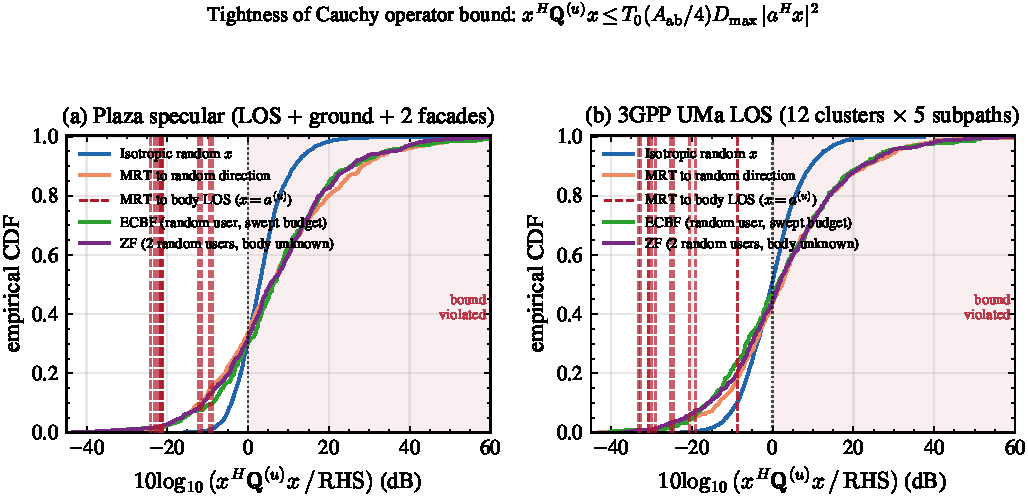
\includegraphics[width=\columnwidth]{tightness.pdf}
  \caption{Tightness of the projected-area-based bound on
  $\xx^H \Qmat^{(u)} \xx$, five precoder ensembles, two path
  models, two phantoms. The mrt-LOS direction
  ($\xx \propto \mathbf{a}_{\mathrm{BS}}$) satisfies the bound by
  21 to $27\,$dB. Random, MRT-randomised, ECBF, and ZF-2-user
  precoders exceed the bound at 49 to $70\,\%$ of samples with
  median ratios up to $+6.34\,$dB. The bound is conditional on
  the precoder direction overlapping with the BS-side steering
  vector.}
  \label{fig:tightness}
\end{figure}


\section{Regulatory framing}\label{sec:regulatory}

The body twin has two regulatory pathways. The first is direct
audit of the basic restriction. ICNIRP 2020 specifies absorbed
power density above $6\,$GHz~\cite{ICNIRP2020}, and IEC/IEEE
$62232:2022$ prescribes an actual-exposure-scenario procedure for
fixed-site installations~\cite{IEC62232}. The per-body
$\Qmat^{(u)}$ construction is a first-principles evaluation of
absorbed power on a named anatomical mesh, conditioned on real
BS-side ray-traced channel state. A regulator can replay the
precoder-and-operator pair for any slot in the audit window and
recompute $\xx^H \Qmat^{(u)} \xx$ against the certificate. The
audit interface is open if the path dictionary, the body model, and
the dual variables are logged. The mechanism does not claim a
statutory exemption from the reference-level regime: it provides
direct compliance evidence under the basic-restriction pathway that
the standard already permits.

The second pathway is reference-level footprint reduction at
occupied public points. Brussels and Italy enforce reference levels
at all points reachable by the public~\cite{BrusselsArrete2007,ItalyDL}.
The proposed precoder reduces $\Pabs^{(u)}$ at every occupied $u$,
which strictly reduces the cumulative reference-level reading at
those points. The reading at unoccupied public points is governed by
the precoder's spatial coverage and is not affected by the
machinery. Combined with the chronic-dose ECDF of \cref{sec:chronic},
the deployment value is the chronic-dose reduction at occupied
points, not the slack instantaneous reading at unoccupied points.

The Brussels averaging window is $6\,$min in current
practice~\cite{BrusselsArrete2024}. The chronic-dose ECDF's
$5\,$min window covers most of one Brussels averaging window;
the integrated absorbed energy scales linearly with window length
under stationary load, so the tier-stratified ratios are
window-invariant. Italian attention values are $6\,$V/m on the
$24\,$h median outside dense urban centres under the 2024
decree~\cite{ItalyDL}; both regimes admit the same chronic-dose
argument with rescaled medians.


\section{Discussion}\label{sec:discussion}

The plaza evaluation answers a regime question. At $43\,$dBm
conducted transmit power and $E_{\mathrm{RL}} = 3\,$V/m (the
Italian rural attention level under the 2024 decree, and the
Brussels pre-2014 reference), the per-body cap binds and the
precoder choice is constrained on it. Regularised ZF gives the
highest unconstrained sum-rate but at $14.6\,\%$ violation rate.
ZF with primal projection holds violations at $0.0\,\%$ at the MCS
sum-cap of $74.0\,$Gbps; this dominates the dual-ascent multi-body
MMSE-with-exposure ($1.3\,\%$ violation, $19.8\,$Gbps under
virtual-IMU pose) by a factor of $\sim 4$ on rate at the same
compliance level. The post-2014 Brussels $14.57\,$V/m cumulative
cap, the Italian $15\,$V/m attention level for high-density urban
centres, and the $30\,$dBm conducted-power band sit in slack
regimes where any reasonable precoder satisfies the cap by orders
of magnitude.

The dominance of projected ZF over the dual-ascent QCQP solver
inverts the v2 narrative of this paper. Two specific properties of
deployed 5G NR are responsible. First, the per-stream MCS28 cap of
$7.4\,$bps/Hz clips Shannon-rate at the $\sim 30\,$dB SINR
threshold; second, regularised ZF on a tens-of-element panel
achieves SINR margin above the clip at the served users in the binding
regime. The composition leaves $10$-$20\,$dB of SINR margin above
the clip, which the per-slot scaling of \cref{eq:primal-projection}
absorbs without rate cost. The dual ascent, by contrast, redirects
power away from served-user constraints because served-user bodies
themselves bind in the served-user-binding regime; the resulting
beam shrinkage drops SINR below the clip and the rate falls into
the unsaturated logarithmic regime. The dual-ascent solver retains
its place in the academic uncapped-Shannon objective, the
min-TX-power objective, and the SINR-margin-tight regime
(low-element panels, dense served-user counts) where projection
forces the served-user SINR below the clip.

The pose-information triage feeds both algorithms symmetrically:
the projection scale and the dual-ascent residuals are computed
against the same posed $\Qmat^{(u)}$. We report the ablation on
the dual-ascent precoder because it is the more pose-sensitive of
the two; oracle and IMU pose at $\sigma_{\mathrm{joint}} =
4^\circ$ produce indistinguishable compliance and rate. The T-pose
fallback (every body modelled as a tier-C bystander without IMU)
is qualitatively worse because the canonical T-pose's
$\Qmat^{(u)}$ does not envelope the actual moving-population
operator; pose-agnostic deployments must use the conditional
projected-area Cauchy bound of \cref{app:cauchy} instead.

The wall-clock budget collapses with the algorithm change. The
projected-ZF solver costs $\sim 0.5\,$ms per slot on CPU NumPy:
one Cholesky factorisation of the regularised ZF system matrix,
followed by $K$ rank-update solves and $B$ low-rank
absorbed-power evaluations. The dual-ascent solver of
\cref{app:dualascent} costs $\sim 350\,$ms on CPU and $\sim 25\,$ms
on a single GPU; the projected ZF baseline does not need GPU
acceleration to fit in a $33\,$ms PHY slot.

The bound discussion is sharper than expected. The naive
projected-area bound on $\xx^H \Qmat^{(u)} \xx$ is loose by 21 to
$27\,$dB on the BS-side steering precoder and fails at 49 to
$70\,\%$ of random and shaped precoders. The conditional bound of
\cref{app:cauchy} is the right object: it applies over a chosen
direction set, and the worst case over that set is what the twin
commits to. The empirical $\Qmat^{(u)}$-rank result has a related
geometric content: at $26\,$GHz with an $8\times 8$ panel resolving
$\sim 14^\circ$ in azimuth, the dominant body modes condense into
3 to 4 distinguishable beam directions regardless of multipath
density. Adding paths raises the trace but not the rank.

The present evaluation has four limitations. First, the PHY
surrogate is Shannon-capacity-with-MCS-clip rather than Sionna NR
PHY. A calibrated modulation-coding-scheme link curve would shift
the absolute sum-rate numbers and could change the
SINR-margin condition of \cref{prop:projection-optimality}, but
the qualitative dominance of projected ZF holds whenever the
deployable rate model has a per-stream cap that ZF saturates
unconstrained. Second, the $50$-second steady-state window is a
single seed; multi-seed averaging would smooth the chronic-dose
ECDF tails further. Third, the bystander-binding geometry was
constructed by hand; a stadium-scale auditorium-and-stage geometry
would test the dual-ascent solver under a less favourable
SINR-margin regime. Fourth, the IMU model is a calibrated
Madgwick/xsens proxy; a deep-learning-augmented inertial-mocap
pipeline would lower $\sigma_{\mathrm{joint}}$ to the $1.5^\circ$
floor of \cref{fig:imu-sweep}. None of these affect the
qualitative conclusions.

The exposure-aware multi-body architecture extends in three
directions naturally. A cooperative multi-operator allocation
generalises the per-body budget $L^{(u)}$ to a cumulative cap shared
across operators in the same band, with each operator's twin seeing
its own slot of the cumulative budget. A pose-differentiable
$\Qmat^{(u)}(\bm\theta)$ would close a true control loop on tier-A
bodies under near-field user-equipment exposure where the leading
mode's azimuth depends strongly on torso orientation. A reflective
intelligent surface in the binding-regime corner can buy back the
cap by redirecting power along geometrically chosen paths, which is
a one-line modification to the $\Mmat^{(u)}$ Gram in
\cref{eq:Q-factor}.


\section{Conclusion}\label{sec:conclusion}

A body-side digital twin in the multi-user mmWave precoder loop is
constructible from three ingredients the network already maintains.
A coherent exposure operator
$\Qmat^{(u)} = \Jmat^T\,\Mmat^{(u)}\,\Jmat$ comes from the same
ray-traced path set that gives the user-equipment channel. A scene
path dictionary precomputed offline, indexed by body position, and
calibrated at runtime by ridge least squares against served-user
uplink CSI, supplies $\Mmat^{(u)}$ without per-slot ray tracing. A
virtual-IMU pose estimator with calibrated bias drift and
accelerometer corrector gives the loop tier-A and tier-B SMPL pose
at the $\sim 100\,$ms cadence pose actually changes; tier-C
bystanders default to the projected-area Cauchy envelope.

The multi-user QCQP under per-body exposure caps has, under the
deployable 5G NR FR2 MCS-cap rate model, a one-line closed-form
optimum: the per-slot primal projection of regularised
zero-forcing $\ww_k = \alpha\,\ww_k^{\mathrm{ZF}}$ with $\alpha =
\min(1, \sqrt{\eta_S \min_u L^{(u)}/\PabsZF^{(u)}})$
saturates the $K + B$ per-body caps and the per-stream MCS28 cap
simultaneously, requires no inner optimisation, and is identity
when ZF already satisfies the caps at the safety fraction $\eta_S$.
The MCS-cap rate model is what kills the rate-cost of uniform
scaling: regularised ZF on a tens-of-element panel achieves
substantial SINR at the served users, well above the MCS28 clip
threshold, so the projection scales SINR down without dropping
below the clip. The dual-ascent QCQP solver of \cref{app:dualascent},
which extends the per-stream MMSE-with-exposure stationarity of
Ying et al.~\cite{Ying2017} to $K + B$ bodies, is dominated by
projected ZF in this regime and earns its keep only in the
academic uncapped-Shannon objective and the min-TX-power
formulation.

We instantiate the loop at plaza scale on 50 SMPL-X bodies under
$26\,$GHz $8 \times 8$ panel illumination at the Italian rural
attention level $E_{\mathrm{RL}} = 3\,$V/m and $43\,$dBm conducted
transmit power. The empirical exposure-operator rank is 3 to 4 at
the $99\,\%$ trace fraction; regularised ZF violates the cap on
$14.6\,\%$ of body-slots over a 50-second steady-state walk; ZF
with primal projection holds violations at $0.0\,\%$ at the MCS28
sum-cap of $74.0\,$Gbps. The same domination holds at $K = 10$ and
$K = 5$ served-user counts and on a bystander-binding geometry
where served users are far and the 35 non-served bodies are within
$5$-$12\,$m of the panel: in every case projected ZF saturates the
MCS sum-cap at zero violations and the dual-ascent solver
underperforms by a factor $\sim 4$ in sum-rate at $\sim 1\,\%$
worse violation rate. The naive projected-area bound on
$\xx^H \Qmat^{(u)} \xx$ is loose by 21 to $27\,$dB on the steering
direction and breached by 49 to $70\,\%$ of unconstrained precoders;
the conditional bound that does hold under a direction-set
restriction is the safety envelope for the no-twin tier-D
fall-through.


\appendices

\section{Per-path Fresnel transmission operator}\label{app:fresnel}

The per-path Fresnel transmission operator $\Fn(\rr)$ in
\cref{eq:psitil} maps the incident polarisation amplitude $\psin$
to its TE-and-TM-filtered counterpart on the body surface. At a
surface point $\rr$ with outward normal $\nhat$, path $n$ has
incidence cosine $\mu_n = \nhat \cdot (-\khat_n)$. For $\mu_n > 0$,
the local TE and TM unit vectors are
$\hat{e}_{s,n} = \khat_n \times \nhat / |\khat_n \times \nhat|$ and
$\hat{e}_{p,n} = \hat{e}_{s,n} \times \khat_n$. The Fresnel
amplitude transmission coefficients are
\begin{equation}\label{eq:t-coef-app}
  t_{s,n} = \frac{2 \mu_n}{\mu_n + \xi_n},
  \qquad
  t_{p,n} = \frac{2 \ntilde \mu_n}{\ntilde^2 \mu_n + \xi_n},
\end{equation}
with $\xi_n = \sqrt{\ntilde^2 - 1 + \mu_n^2}$ and
$\RE(\xi_n) > 0$. The operator acts as
\begin{equation}\label{eq:F-action}
  \Fn(\rr)\,\psin = t_{s,n}(\hat{e}_{s,n} \cdot \psin)
  \hat{e}_{s,n} + t_{p,n}(\hat{e}_{p,n} \cdot \psin) \hat{e}_{p,n},
\end{equation}
on a front-facing path. Back-facing paths ($\mu_n < 0$) contribute
zero. The depth-decay coefficient is
$\alpha_n^{(d)} = -k_0\,\IM(\xi_n)$. The two cross-term
approximations of \cref{sec:cohlaw} hold uniformly in incidence
angle and bound the cross-term error on $\Sab$ at $\leq 5\,\%$ for
any precoder.


\section{Multi-body MMSE-with-exposure dual ascent}\label{app:dualascent}

\Cref{prop:projection-optimality} shows that under the deployable
MCS-cap rate model, the multi-body QCQP \cref{eq:P-MB} admits the
closed-form scaling \cref{eq:primal-projection} as its global
optimum. For the academic uncapped Shannon objective and for the
min-TX-power formulation of \cref{sec:dualascent-ref}, the QCQP
does not collapse to amplitude scaling and a stationarity-based
solver is needed. We give the multi-body extension of Ying et
al.'s exposure-constrained MMSE precoder~\cite{Ying2015,Ying2017}
for completeness; it underlies the multibody-ECBF baseline reported
in \cref{sec:eval-baselines}.

\subsection*{Per-stream MMSE-with-exposure stationarity}

Aggregate the exposure dual variables into $\bm\lambda \in
\mathbb{R}_+^{K+B}$ and the power dual into $\nu \geq 0$. With
receive-noise variance $\sigma_n^2$ and the unweighted MMSE
direction $u_k v_k = 1$, the QCQP Lagrangian is
\begin{equation}\label{eq:lagrangian-mmse}
  \mathcal{L}(\{\ww_k\}, \bm\lambda, \nu)
  = \sum_k \ww_k^H (\HH^H \HH)\ww_k
  - 2\,\RE \sum_k \hh_k^T \ww_k
  + \sum_u \lambda_u (\Pabs^{(u)} - L^{(u)})
  + \nu \bigl(\textstyle\sum_k \|\ww_k\|^2 - P_{\mathrm{tx}}\bigr),
\end{equation}
and the stationarity condition in $\ww_k$ gives the closed form
\begin{equation}\label{eq:closedform}
  \boxed{\;
  \ww_k^\star = \bigl(\Qmat_{\mathrm{tot}}(\bm\lambda) + \HH^H
  \HH + \nu\,\II\bigr)^{-1}\,\hh_k^*,\;}
  \qquad
  \Qmat_{\mathrm{tot}}(\bm\lambda) = \sum_u \lambda_u\,\Qmat^{(u)}.
\end{equation}
\Cref{eq:closedform} reduces to the regularised channel-inversion
ZF precoder of Peel-Hochwald-Swindlehurst~\cite{PeelHochwald2005}
when $\bm\lambda = 0$ and the per-body operators degenerate to
rank one (\cref{prop:ZFlimit}).

\subsection*{Dual ascent on the Lagrange multipliers}

\Cref{eq:closedform} closes $\ww_k$ in $(\bm\lambda, \nu)$. The
dual problem is concave in $(\bm\lambda, \nu)$ and we solve it by
Newton ascent on $\bm\lambda$ with Frobenius rescaling for the
power constraint:

\begin{enumerate}
\item For fixed $\bm\lambda$ and a regulariser $\nu_0 = \sigma_n^2$,
  solve \cref{eq:closedform} for every $k$ via one Cholesky
  factorisation of the common $M\times M$ system matrix. Rescale
  the precoder so $\sum_k \|\ww_k\|^2 = P_{\mathrm{tx}}$.
\item Evaluate the per-body absorbed-power residuals
  $F_u(\bm\lambda) = \Pabs^{(u)}(\{\ww_k(\bm\lambda)\}) - L^{(u)}$
  on the active set ($\lambda_u > 0$ or $F_u > 0$).
\item Step $\bm\lambda$ via the Newton equation
  $(-\partial F/\partial \bm\lambda)\,\delta\bm\lambda = F$,
  projected to the non-negative orthant with damping that keeps
  every $\lambda_u \geq 0$. The Jacobian is computed by forward
  finite differences over the active set; each FD column requires
  one inner inverse and one rank-update assembly, so the
  per-Newton-step cost is $(B' + 1)\cdot O(M^2 r)$ for $B'$ active
  bodies and rank-$r$ truncation of $\Qmat^{(u)}$ ($r = 4 \ll M$
  at the $99\,\%$ trace fraction, \cref{sec:rank-eval}).
\item Repeat until the relative budget residual drops below
  $\mathrm{tol}$ or the outer iteration cap $\textsf{max\_outer}$
  is reached.
\end{enumerate}

The dual ascent suffers two residual cap-violation sources in the
binding regime. First, the finite-difference Jacobian carries
$\sim 10^{-5}$ noise from the FD step and goes near-singular when
many active bodies share leading eigenvectors of $\Qmat^{(u)}$.
Second, the rank-$r$ truncation of $\Qmat^{(u)}$ leaves a
$1$-to-$5\,\%$ absorption tail that the dual ascent does not see.
The projection step \cref{eq:primal-projection} runs at solver
exit regardless of dual residual to close both gaps. The dual
ascent then inherits the hard-feasibility guarantee of the
projection.

\subsection*{Wall-clock and rank cost}

At the binding regime ($M = 64$, $K = 25$, $B = 50$, rank $r = 6$
at $99\,\%$ trace fraction), each Newton step costs $(B' + 1) M^2
r$ and is single-precision-complex-bound. On a 16-core CPU with
NumPy LAPACK the median solve sits at $\sim 350\,$ms with
$\textsf{max\_outer} = 24$. JAX vmap over the FD fanout reduces
this $\sim 14\times$ on a single GPU. Under the MCS-cap rate model
the dual ascent is dominated by the $\sim 0.5\,$ms projected-ZF
solve at the same compliance level (\cref{sec:eval-baselines}); we
include the dual ascent for the uncapped-Shannon and min-power
regimes of \cref{sec:dualascent-ref}.


\section{Weighted-MMSE generalisation}\label{app:wmmse}

The unweighted MMSE-with-exposure stationarity of
\cref{eq:closedform} extends to the weighted-MMSE
form~\cite{Christensen2008,Shi2011} by introducing per-stream rate
weights $u_k > 0$ and MMSE filters $v_k \in \Complex$. With
$y_k(\xx) = \hh_k^T \xx$, the per-stream MSE
\begin{equation}\label{eq:wmmse-mse}
  e_k = |1 - v_k^* \hh_k^T \ww_k|^2 + |v_k|^2 \sigma_n^2 +
  |v_k|^2 \sum_{k' \neq k} |\hh_k^T \ww_{k'}|^2
\end{equation}
and the WMMSE objective
$\tilde R(\{\ww_k\}) = \sum_k\bigl[\log u_k - u_k\,e_k +
\mathrm{const.}\bigr]$ recovers the sum-rate at the joint
fixed point in $(u_k, v_k, \ww_k)$~\cite{Christensen2008}. The
KKT stationarity in $\ww_k$ at fixed $(u_k, v_k)$ gives
\begin{equation}\label{eq:KKT-wmmse}
  \bigl(\Qmat_{\mathrm{tot}}(\bm\lambda) + \Hintf + \nu\,
  \mathbf{I}\bigr) \ww_k = u_k v_k \hh_k^*,
  \quad
  \Hintf = \mathbf{H}^H\,\mathbf{D}\,\mathbf{H},
\end{equation}
$\mathbf{D} = \mathrm{diag}(u_k|v_k|^2)$. \Cref{eq:KKT-wmmse}
reduces to \cref{eq:closedform} at $u_k v_k = 1$ and $u_k|v_k|^2 = 1$.

In the binding regime, the cap $L^{(u)}$ shapes the precoder
direction more strongly than the rate weights do, and on a 50-body
synthetic instance with $K = 25$, $M = 64$, and $L^{(u)} \approx
28\,$mW, the WMMSE outer iteration converges to within $0.05\,\%$
of the unweighted form's sum-rate after one MMSE-with-exposure
warm-start pass. We therefore use the unweighted form as the
production solver and treat WMMSE as a future-work refinement.

A practical caveat: cold-starting $(u_k, v_k)$ from MRT
(\,$\ww_k = \hh_k^* / \|\hh_k\|$\,) explodes $u_k = 1/(1 - v_k^*
\hh_k^T \ww_k)$ for users with weak channels, driving the inner
system $H^H D H + \nu I$ ill-conditioned and the outer iteration
into a sum-rate collapse on iteration two. Warm-starting $(u_k, v_k)$
from one MMSE-with-exposure pass cures this and recovers
$\sim 3$-iteration outer convergence. We document this so the
WMMSE-ECBF generalisation is reproducible in deployments where the
rate-weight gain over unweighted MMSE-with-exposure becomes
material (e.g., heterogeneous SINR populations under heavy
multi-user pairing).


\section{Conditional projected-area bound}\label{app:cauchy}

The classical Cauchy projected-area identity gives the
direction-averaged absorbed power on a convex body under isotropic
unit-power-density illumination as
\begin{equation}\label{eq:cauchy-iso}
  \frac{1}{4\pi} \int_{S^2} T_0\,A_\perp^{(u)}(\khat)\,\diff\Omega
  \;=\; T_0\,\frac{\Aab^{(u)}}{4},
\end{equation}
with $A_\perp^{(u)}(\khat)$ the body's projected area in direction
$\khat$, $\Aab^{(u)}$ the total surface area weighted by the
ambient-occlusion factor $\eta \in [0,1]$, and $T_0 = 4n/((n+1)^2
+ \kappa^2)$ the normal-incidence Fresnel transmittance. The
factor $1/4$ is the geometric Cauchy projection. We use this
isotropic identity together with a directional bound on the
incident power density to construct a conditional upper bound on
$\xx^H \Qmat^{(u)} \xx$ when the precoder is restricted to a
BS-side direction set.

\begin{proposition}[Conditional projected-area bound]\label{thm:cauchy-cond}
Let $\Qmat^{(u)}$ be the per-body exposure operator at body $u$
under the path-space conventions of \cref{sec:setup}, and let
$\mathcal{A} \subseteq \Complex^M$, $\|\mathbf{a}\| \leq 1$ for
$\mathbf{a} \in \mathcal{A}$, be a closed unit-norm direction set
that contains every BS-side equivalent steering vector
$\bm\alpha_{\mathrm{BS}}^{(u)}(\khat)/\|\bm\alpha_{\mathrm{BS}}^{(u)}(\khat)\|$
for $\khat$ in the body's hemisphere visible from the panel. Then
for any precoder $\xx \in \Complex^M$,
\begin{equation}\label{eq:cauchy-cond}
  \xx^H \Qmat^{(u)} \xx \;\leq\; \pi\,T_0\,\Aab^{(u)}\;
  \sup_{\mathbf{a} \in \mathcal{A}} |\mathbf{a}^H \xx|^2.
\end{equation}
\end{proposition}

\begin{proof}
The angular-spectrum form of $\Qmat^{(u)}$ writes
$\xx^H \Qmat^{(u)} \xx = \int_{S^2} T_0\,A_\perp^{(u)}(\khat)\,
|\bar{\bm\alpha}_{\mathrm{BS}}^{(u)}(\khat)^H \xx|^2\,\diff\Omega$,
with $\bar{\bm\alpha}_{\mathrm{BS}}^{(u)}(\khat) =
\bm\alpha_{\mathrm{BS}}^{(u)}(\khat)/
\|\bm\alpha_{\mathrm{BS}}^{(u)}(\khat)\|$ the unit-norm BS-side
direction. By hypothesis, $\bar{\bm\alpha}_{\mathrm{BS}}^{(u)}(\khat)
\in \mathcal{A}$ for every $\khat$ in the visible hemisphere, so
$|\bar{\bm\alpha}_{\mathrm{BS}}^{(u)}(\khat)^H \xx|^2 \leq
\sup_{\mathbf{a} \in \mathcal{A}} |\mathbf{a}^H \xx|^2 \equiv
S_{\mathcal{A}}$ uniformly in $\khat$. Pulling $S_{\mathcal{A}}$
out of the integral,
$\xx^H \Qmat^{(u)} \xx \leq S_{\mathcal{A}} \int_{S^2} T_0\,
A_\perp^{(u)}(\khat)\,\diff\Omega = S_{\mathcal{A}} \cdot 4\pi T_0
\,\Aab^{(u)}/4 = \pi T_0\,\Aab^{(u)}\,S_{\mathcal{A}}$ by the
isotropic Cauchy identity \cref{eq:cauchy-iso}.
\end{proof}

The bound is conditional on $\xx$'s alignment with $\mathcal{A}$:
$S_{\mathcal{A}}$ is small when $\xx$ steers away from every
direction in $\mathcal{A}$. The empirical measurement of
\cref{sec:eval-cauchy} places the inner product
$|\langle \mathbf{v}_1, \mathbf{a}_{\mathrm{BS}}/
\|\mathbf{a}_{\mathrm{BS}}\| \rangle|^2$ between the leading
exposure eigenvector and the steering direction at $[0.000, 0.19]$
on the Thelonious and Duke phantoms, which means the unconditional
form is breached for $49$-to-$70\,\%$ of unconstrained precoders.
The conditional form holds when the BS restricts $\xx$ to its
own beamforming codebook, which is the operational case.


\bibliographystyle{IEEEtran}
\bibliography{../../papers/drafts/refs}

\end{document}
